\documentclass[12pt]{article}
\usepackage{amsmath}
\usepackage{amsthm}
\usepackage{amssymb}
\usepackage{euscript}
\usepackage{mathrsfs}
\usepackage{bm}
\usepackage{enumitem}
\usepackage{tikz}
\usepackage{mathtools}
\usepackage{float}
\usepackage{hyperref}
\usepackage{boldline}
\usepackage{indentfirst}
\usepackage{environ}
\usepackage{courier}
\usetikzlibrary{positioning}

\renewcommand{\labelitemii}{$\vartriangleright$}
\renewcommand{\labelitemiv}{$\Join$}

\makeatletter
\newsavebox{\measure@tikzpicture}
\NewEnviron{scaletikzpicturetowidth}[1]{%
  \def\tikz@width{#1}%
  \def\tikzscale{1}\begin{lrbox}{\measure@tikzpicture}%
  \BODY
  \end{lrbox}%
  \pgfmathparse{#1/\wd\measure@tikzpicture}%
  \edef\tikzscale{\pgfmathresult}%
  \BODY
}
\makeatother

\numberwithin{equation}{section}

\hypersetup{
    colorlinks=true,
    % linkcolor=blue,
    linkcolor=[RGB]{0,0,128},
    % filecolor=[RGB]{0,0,128},
    filecolor=magenta,
    urlcolor=cyan,
    citecolor = [RGB]{128,0,128}
}

\newcommand{\myref}[2]{\hyperref[#2]{#1 \ref*{#2}}}
\newcommand{\myrefT}[1]{\hyperref[#1]{Theorem \ref*{#1}}}
\newcommand{\myrefP}[1]{\hyperref[#1]{Proposition \ref*{#1}}}
\newcommand{\myrefL}[1]{\hyperref[#1]{Lemma \ref*{#1}}}
\newcommand{\myrefD}[1]{\hyperref[#1]{Definition \ref*{#1}}}
\newcommand{\myrefn}[3]{\hyperref[#2]{#1 \ref*{#2} (#3)}}

% \input{dynkinMacros.tex}
% \input{dynkinEMacros.tex}
% \renewcommand{\qedsymbol}{}
\newcommand{\ssm}{\smallsetminus}

\newcommand{\para}[1]{\noindent\underline{#1}.}

\newcommand{\ti}{$\tau\textnormal{-invariant}$}
\newcommand{\prim}{\textnormal{Prim}_{\lambda}(\textnormal{U}(\gf))}

\newcommand{\ve}{\varepsilon}
\newcommand{\veo}{\varepsilon_1}
\newcommand{\vet}{\varepsilon_2}
\newcommand{\vei}{\varepsilon_i}
\newcommand{\vp}{\varphi}

% \newcommand{\inr}{\textnormal{In}^R}
% \newcommand{\inl}{\textnormal{In}^L}
% \newcommand{\inc}{\textnormal{In}}
% \renewcommand{\sc}{\textnormal{SC}}
% \newcommand{\re}{\textnormal{Re}}

\newcommand{\ag}{\alpha}
\newcommand{\bg}{\beta}
\newcommand{\g}{\gamma}
\newcommand{\dg}{\delta}
\newcommand{\rg}{\rho}
\newcommand{\kg}{\kappa}
\newcommand{\sg}{\sigma}
\newcommand{\tg}{\tau}
\renewcommand{\lg}{\lambda}

\renewcommand{\gg}{$\gamma \ $}
\newcommand{\ga}{$\alpha \ $}
\newcommand{\gt}{$\tau $}
\renewcommand{\(}{(\gamma)}
\newcommand{\atg}{\tilde\alpha}
\newcommand{\ags}[1]{{\ag_{#1}}}
\newcommand{\ao}{{\ag_1'}}

\newcommand{\gf}{\mathfrak g}
\newcommand{\hf}{\mathfrak h}

% needs a new name
%\newcommand{\th}[1]{{$\text{\it #1 }^{\underline{\textnormal{th}}}$}}
\renewcommand{\sf}{\mathscr F}
\newcommand{\dsf}{$\sf$}
\newcommand{\st}{\mathscr T}
% needs a new name  -- ok?
\newcommand{\so}[1]{\mathscr #1}


\newcommand{\snn}{{\mathscr S(n,n)}}
\newcommand{\smm}{{\mathscr S(M^L,M^R)}}
\renewcommand{\tan}{\mathscr T_A(n)}
\newcommand{\tn}{\mathscr T(n)}
\newcommand{\dtn}{$\tn$}
\newcommand{\tm}{\mathscr T(M)}
\newcommand{\dtm}{$\tm$}
\newcommand{\tcsn}{\mathscr T_C^S(n)}
\newcommand{\tbsn}{\mathscr T_B^S(n)}
\newcommand{\tsn}[1]{\mathscr T_#1(n)}
\newcommand{\tsm}[1]{\mathscr T_#1(M)}
\newcommand{\tnn}{\mathscr T(n,n)}
\newcommand{\tmm}{\mathscr T(M^L,M^R)}
\newcommand{\tkmm}{\mathscr T_K(M^L,M^R)}
\newcommand{\tsnn}[1]{\mathscr T_#1(n,n)}
\newcommand{\tsmm}[1]{\mathscr T_#1(M^L,M^R)}
\newcommand{\tdnn}{\mathscr T_D(n,n)}
\newcommand{\tdmm}{\mathscr T_D(M^L,M^R)}
\newcommand{\tdn}{\mathscr T_D(n)}
\newcommand{\tdm}{\mathscr T_D(M)}
\newcommand{\tcnn}{\mathscr T_C(n,n)}
\newcommand{\tcmm}{\mathscr T_C(M^L,M^R)}
\newcommand{\tcn}{\mathscr T_C(n)}
\newcommand{\tcm}{\mathscr T_C(M)}
\newcommand{\cm}{\mathscr C(M)}
\newcommand{\dm}{\mathscr D(M)}

\newcommand{\snnp}{\mathscr S'(n,n)}
\newcommand{\smmp}{\mathscr S'(M^L,M^R)}
\newcommand{\snnpp}{\mathscr S''(n,n)}
\newcommand{\smmpp}{\mathscr S''(M^L,M^R)}
\newcommand{\tnnp}{\mathscr T'(n,n)}
\newcommand{\tmmp}{\mathscr T'(M^L,M^R)}
\newcommand{\tnnpp}{\mathscr T''(n,n)}
\newcommand{\tmmpp}{\mathscr T''(M^L,M^R)}
\newcommand{\tdnnp}{\mathscr T_D'(n,n)}
\newcommand{\tdmmp}{\mathscr T_D'(M^L,M^R)}
\newcommand{\tdnnpp}{\mathscr T_D''(n,n)}
\newcommand{\tdmmpp}{\mathscr T_D''(M^L,M^R)}


\newcommand{\talb}{T_{\alpha \beta}}
\newcommand{\tai}{T_{\alpha_i,\alpha_{i+1}}}
\newcommand{\tap}{T_{\alpha_{i+1},\alpha_i}}
\newcommand{\tao}{T_{\alpha_1,\alpha_2}}
\newcommand{\tat}{T_{\alpha_2,\alpha_1}}

% new
\newcommand{\talbLeft}{T^L_{\alpha \beta}}
\newcommand{\talbRight}{T^R_{\alpha \beta}}

\newcommand{\ot}{\overline T}
\newcommand{\og}{\overline{\gamma}}

\newcommand{\sij}{{S_{ij}}}
\renewcommand{\ss}[2]{{S_{#1,#2}}}
% \def\ss#1#2{S_{#1,#2}}

\newcommand{\im}{{i-1}}
% \renewcommand{\ip}{{i+1}}
\newcommand{\ip}{{i+1}}
\newcommand{\imm}{{i-2}}
\newcommand{\ipp}{{i+2}}
\newcommand{\jm}{{j-1}}
\newcommand{\jp}{{j+1}}
\newcommand{\jmm}{{j-2}}
\newcommand{\jpp}{{j+2}}

\renewcommand{\tt}{\tau (T)}
\newcommand{\abe}{{$\{\ag,\bg\}=\{\ag_i,\ag_\ip\}$}}

\newcommand{\bt}{\mathbf T}
\newcommand{\bto}{\mathbf T_1}
\newcommand{\btt}{\mathbf T_2}
\newcommand{\obt}{\overline\bt}
\newcommand{\obto}{\overline\bt_1}
\newcommand{\obtt}{\overline\bt_2}
\newcommand{\tbt}{\tilde\bt}
\newcommand{\tbto}{\tilde\bto}
\newcommand{\tbtt}{\tilde\btt}
\newcommand{\pbt}{(\bto,\btt)}
\newcommand{\pbtp}{(\bto',\btt')}
\newcommand{\pobt}{(\obto,\obtt)}
\newcommand{\pbts}[1]{(\bto^{#1},\btt^{#1})}
\newcommand{\pobts}[1]{(\obto^{#1},\obtt^{#1})}
\newcommand{\pobtp}{(\obto',\obtt')}

\newcommand{\lo}{(\bto,\bt)}
\newcommand{\lop}{(\bto',\bt)}
\newcommand{\ls}[1]{(\bt_#1,\bt)}
\newcommand{\lsp}[1]{(\bt_#1',\bt)}
\newcommand{\ol}{(\obt_1,\obt)}

\newcommand{\be}{\mathbf E}
\newcommand{\bs}{\mathbf S}
\newcommand{\bl}{\mathbf L}
\newcommand{\br}{\mathbf R}
% \renewcommand{\op}{\bar P}
\newcommand{\op}{\bar P}
\newcommand{\pe}{P_e}

\newcommand{\oc}{\overline c}
\newcommand{\cL}{\prescript{L}{}{c}}
\newcommand{\cR}{\prescript{R}{}{c}}
\newcommand{\bc}{\mathbf c}
\newcommand{\bcL}{\prescript{L}{}{\bc}}
\newcommand{\bcR}{\prescript{R}{}{\bc}}
\newcommand{\overbc}{\overline{\mathbf c}}
\newcommand{\overcL}{\prescript{L}{}{\overline c}}
\newcommand{\overcR}{\prescript{R}{}{\overline c}}
\newcommand{\overbcL}{\prescript{L}{}{\overbc}}
\newcommand{\overbcR}{\prescript{R}{}{\overbc}}

% \newcommand{\sha}{{\textnormal{Shape}}}
\newcommand{\cs}{{c.s.p.b.}}
% \newcommand{\OC}{{\textnormal{OC}}}
% \newcommand{\OCS}{{\textnormal{OC*}}}
\newcommand{\Sf}{S_f}
\newcommand{\Sb}{S_b}
\newcommand{\nh}{n_h}
\newcommand{\nv}{n_v}
\newcommand{\rinf}{\rg_{\inf}}
\newcommand{\rsup}{\rg_{\sup}}

\newcommand{\ec}{\underset {ec}\sim}
\newcommand{\gtl}{\underset {GTL}\sim}
\newcommand{\en}{\underset {n}\sim}
\newcommand{\enm}{\underset {n-1}\sim}
\newcommand{\eqm}{\underset {m}\sim}
\newcommand{\eqmm}{\underset {m-1}\sim}
\newcommand{\ez}{\underset {0}\sim}
\newcommand{\gtr}{\underset {GTR}\sim}
\renewcommand{\gt}{\underset {GT}\sim}
\newcommand{\ngtl}{\underset {GTL}\nsim}
\newcommand{\jl}{\underset {JL}\sim}
\newcommand{\jr}{\underset {JR}\sim}
\newcommand{\kll}{\underset {KLL}\sim}
\newcommand{\klr}{\underset {KLR}\sim}

\newcommand{\fo}{F_1}
\newcommand{\ft}{F_2}
\newcommand{\fot}{\tilde\fo}
\newcommand{\ftt}{\tilde\ft}

\newcommand{\bi}{{\it b}){\it i})}
\newcommand{\bii}{{\it b}){\it ii})}

\newcommand{\sig}{\Sigma}
\newcommand{\tsl}{T_\Sigma^L}
\newcommand{\tspl}{T_{\Sigma'}^L}
\newcommand{\tssl}[1]{T_{\Sigma^#1}^L}
\newcommand{\tssbl}[1]{T_{\Sigma_#1}^L}
\newcommand{\ts}{T_\Sigma}
\newcommand{\tsp}{T_{\Sigma'}}
\newcommand{\tss}[1]{T_{\Sigma^#1}}
\newcommand{\tssb}[1]{T_{\Sigma_#1}}
\newcommand{\pin}{$\Pi\ssm\{\ag_n\}$}
\newcommand{\pc}{\phi_C}
% \newcommand{\pd}{{\phi_D}}
\newcommand{\il}{I_\lg}

\newcommand{\te}[1]{\textnormal{#1}}

\newcommand{\plainTL}{\prescript{L}{}{T}}
\newcommand{\plainTR}{\prescript{R}{}{T}}

\newcommand{\tL}{\prescript{L}{}{\bt}}
\newcommand{\tR}{\prescript{R}{}{\bt}}
\newcommand{\pairTLR}{(\tL,\tR)}
\newcommand{\pairTLRPrime}{(\tL',\tR')}
\newcommand{\pairTLRSub}[1]{(\tL_{#1},\tR_{#1})}
\newcommand{\pairTLRPrimeSub}[1]{(\tL'_{#1},\tR'_{#1})}

\newcommand{\overTL}{\prescript{L}{}{\obt}}
\newcommand{\overTR}{\prescript{R}{}{\obt}}
\newcommand{\overPairTLR}{(\overTL,\overTR)}
\newcommand{\overPairTLRPrime}{(\overTL',\overTR')}
\newcommand{\overPairTLRSub}[1]{(\overTL_{#1},\overTR_{#1})}
\newcommand{\overPairTLRPrimeSub}[1]{(\overTL'_{#1},\overTR'_{#1})}

\newcommand{\tildeTL}{\prescript{L}{}{\tbt}}
\newcommand{\tildeTR}{\prescript{R}{}{\tbt}}
\newcommand{\tildePairTLR}{(\tildeTL, \tildeTR)}
\newcommand{\pairTLRStar}{(\tL^*, \tR^*)}
\newcommand{\overPairTLRStar}{(\overTL^*, \overTR^*)}

\newcommand{\pisn}{{$\Pi^*\ssm\{\ag_n\}$}}

\newcommand{\tLSigma}{\tsl}
\newcommand{\tLSigmaSub}[1]{\tssbl#1}
\newcommand{\tDMM}{\tdmm}

\newcommand{\leftPrime}{(\tL',\tR)}
\newcommand{\leftSub}[1]{(\tL_{#1},\tR)}
\newcommand{\leftPrimeSub}[1]{(\tL_{#1}',\tR)}


\DeclareMathOperator{\Shape}{Shape}
\DeclareMathOperator{\OC}{OC}
\DeclareMathOperator{\OCS}{OC*}
% \newcommand{\inr}{\textnormal{In}^R}
% \newcommand{\inl}{\textnormal{In}^L}
% \newcommand{\inc}{\textnormal{In}}
% \renewcommand{\sc}{\textnormal{SC}}
\newcommand{\re}{\textnormal{Re}}
\DeclareMathOperator{\In}{In}
\newcommand{\inc}{\In}
\newcommand{\inL}{\In^L}
\newcommand{\inR}{\In^R}
\DeclareMathOperator{\SC}{SC}
\newcommand{\scL}{\SC^L}
\newcommand{\scR}{\SC^R}

\DeclareMathOperator{\Adj}{Adj}
\newcommand{\oeta}{\overline{\eta}}

\newcommand{\preL}[1]{\prescript{L}{}{#1}}

\newcommand{\makeBox}[2] {
  \newsavebox{#1}
  \begin{lrbox}{#1}{#2}\end{lrbox}
}

\tikzstyle{tableau} = [y = -1cm, every node/.style={transform shape}]

\definecolor{gridColor}{RGB}{19,83,150}
\tikzstyle{dominoStyle} = [color=black, fill=white, rounded corners = .1cm, thick]
\tikzstyle{gridLine} = [color=gridColor, thick]
\tikzstyle{dominoText} = [font=\Large, midway]
\tikzstyle{cycleLine} = [color=green, thick, >->]
\tikzstyle{closedCycleLine} = [color=green, thick]
% \tikzstyle{fixedSquareStyle} = [pattern = crosshatch doats, pattern color=gridColor,  opacity=0.2]
\tikzstyle{fixedSquareStyle} = [color=gridColor,  opacity=0.07]
\tikzstyle{tileText} = [font=\large, midway]

\newcommand{\eps}{.06}
\newcommand{\teps}{\eps * 2}

% first entry is row, starting with 1, second entry is column, third is content
\newcommand{\filledSquare}[3]{\filldraw [dominoStyle] (#2 - 1 + \eps, #1 - 1 + \eps) rectangle + (1 - \teps, 1 -\teps) node [tileText] {$#3$};}
% The fourth entry shifts vertically
\newcommand{\filledSquareShift}[4]{\filldraw [dominoStyle] (#2 - 1 + #4 + \eps, #1 - 1 + \eps) rectangle + (1 - \teps, 1 -\teps) node [tileText] {$#3$};}

\newcommand{\horizontalDomino}[3]{\filldraw [dominoStyle] (#2 - 1 + \eps, #1 - 1 + \eps) rectangle + (2 - \teps, 1 -\teps) node [dominoText] {$#3$};}
\newcommand{\verticalDomino}[3]{\filldraw [dominoStyle] (#2 - 1 + \eps,  #1 - 1 + \eps) rectangle + (1 - \teps,2 -\teps) node [dominoText] {$#3$};}

\newcommand{\horizontalDominoShift}[4]{\filldraw [dominoStyle] (#2 - 1 + #4 + \eps, #1 - 1 + \eps) rectangle + (2 - \teps, 1 -\teps) node [dominoText] {$#3$};}
\newcommand{\verticalDominoShift}[4]{\filldraw [dominoStyle] (#2 - 1 + #4 + \eps,  #1 - 1 + \eps) rectangle + (1 - \teps,2 -\teps) node [dominoText] {$#3$};}

\newcommand{\zeroSquare}[2]{\filldraw [dominoStyle] (#2 - 1 + \eps, #1 - 1 + \eps) rectangle + (1 - \teps, 1 -\teps) node [dominoText] {$0$};}
\newcommand{\zeroSquareShift}[3]{\filldraw [dominoStyle] (#2 - 1 + #3 + \eps, #1 - 1 + \eps) rectangle + (1 - \teps, 1 -\teps) node [dominoText] {$0$};}


\newcommand{\emptyBox}[2]{\filldraw [dominoStyle] (#2 - 1 + \eps, #1 - 1 + \eps) rectangle + (2 - \teps, 2 -\teps);}
\newcommand{\signedBox}[3]{
\filldraw [opacity=0] (#2 - 1 + 1, #1 - 1) rectangle + (1, 2) node [dominoText,opacity=1] {$#3$};
\filldraw [dominoStyle, fill opacity = 0] (#2 - 1 + \eps, #1 - 1 + \eps) rectangle + (2 - \teps, 2 -\teps);
}

\newcommand{\emptyBoxShift}[3]{\filldraw [dominoStyle] (#2 - 1 + #3 + \eps, #1 - 1 + \eps) rectangle + (2 - \teps, 2 -\teps);}
\newcommand{\signedBoxShift}[4]{
\filldraw [opacity=0] (#2 - 1 + 1 + #4, #1 - 1) rectangle + (1, 2) node [dominoText,opacity=1] {$#3$};
\filldraw [dominoStyle, fill opacity = 0] (#2 - 1 + #4 + \eps, #1 - 1 + \eps) rectangle + (2 - \teps, 2 -\teps);
}

% These rows and columns are zero-based
\newcommand{\horizontalGridLine}[3]{\draw [gridLine] (#1, #2) -- + (#3,0);}
\newcommand{\verticalGridLine}[2]{\draw [gridLine] (#1, 0) -- + (0,#2);}
\newcommand{\fixedSquare}[2]{\filldraw [fixedSquareStyle] (#1,#2) rectangle +(1,1);}

% This will have #1 * 2 rows and #2 *2 columns
\newcommand{\gridLines}[2] {
  \pgfmathsetmacro{\verticalEnd}{2 * #1}
  \pgfmathsetmacro{\horizontalEnd}{2 * #2}
  \foreach \vertical in {0,...,#2} {
    \pgfmathsetmacro{\var} {2 * \vertical}
    \verticalGridLine{\var}{\verticalEnd}
  }
  \foreach \horizontal in {0,...,#1} {
    \pgfmathsetmacro{\var} {2 * \horizontal}
    \horizontalGridLine{0}{\var}{\horizontalEnd}
  }
}

% This will have #1 * 2 rows and #2 *2 columns
% The vertical lines will be shifted over #3 squares
\newcommand{\gridLinesShift}[3] {
  \pgfmathsetmacro{\verticalEnd}{2 * #1}
  \pgfmathsetmacro{\horizontalEnd}{2 * #2}
  \foreach \vertical in {0,...,#2} {
    \pgfmathsetmacro{\var} {2 * \vertical + #3}
    \verticalGridLine{\var}{\verticalEnd}
  }
  \foreach \horizontal in {0,...,#1} {
    \pgfmathsetmacro{\var} {2 * \horizontal}
    \horizontalGridLine{#3}{\var}{\horizontalEnd}
  }
}

\newcommand{\fixedSquaresStart}[4]{
  \foreach \row in {#1,...,#2} {
    \foreach \column in {#3,...,#4} {
      \pgfmathsetmacro{\var}{\row + \column}
      \ifodd \var
      \else
        \fixedSquare\column\row
      \fi
    }
  }
}

\newcommand{\fixedSquares}[2]{
  \foreach \row in {0,...,#1} {
    \foreach \column in {0,...,#2} {
      \pgfmathsetmacro{\var}{\row + \column}
      \ifodd \var
        \fixedSquare\column\row
      \fi
    }
  }
}

% This has #1 * 2 rows and #2 * 2 columns
\newcommand{\fixedSquaresForGrid}[2] {
  \pgfmathsetmacro{\rowParameter}{#1 * 2 - 1}
  \pgfmathsetmacro{\columnParameter}{#2 * 2 - 1}
  \fixedSquares{\rowParameter}{\columnParameter}
}

% This has #1 * 2 rows and #2 * 2 columns
% The vertical lines will be shifted over #3 squares
\newcommand{\fixedSquaresForGridShift}[3] {
  \pgfmathsetmacro{\rowParameter}{#1 * 2 - 1}
  \pgfmathsetmacro{\columnStart}{#3}
  \pgfmathsetmacro{\columnEnd}{#2 * 2 - 1 + #3}
  \fixedSquaresStart{0}{\rowParameter}{\columnStart}{\columnEnd}
}

\newcommand{\fixedSquaresStartAlt}[4]{
  \foreach \row in {#1,...,#2} {
    \foreach \column in {#3,...,#4} {
      \pgfmathsetmacro{\var}{\row + \column + 1}
      \ifodd \var
      \else
        \fixedSquare\column\row
      \fi
    }
  }
}

% This has #1 * 2 rows and #2 * 2 columns
% The vertical lines will be shifted over #3 squares
\newcommand{\fixedSquaresForGridShiftAlt}[3] {
  \pgfmathsetmacro{\rowParameter}{#1 * 2 - 1}
  \pgfmathsetmacro{\columnStart}{#3}
  \pgfmathsetmacro{\columnEnd}{#2 * 2 - 1 + #3}
  \fixedSquaresStartAlt{0}{\rowParameter}{\columnStart}{\columnEnd}
}


% This will have #1 rows and #2 columns
\newcommand{\typeAGridLines}[2] {
  \foreach \vertical in {0,...,#2} {
    \verticalGridLine{\vertical}{#1}
  }
  \foreach \horizontal in {0,...,#1} {
    \horizontalGridLine{0}{\horizontal}{#2}
  }
}

% This will have #1 rows and #2 columns
% The vertical lines will be shifted over #3 squares
\newcommand{\typeAGridLinesShift}[3] {
  \foreach \vertical in {0,...,#2} {
    \pgfmathsetmacro{\var} {\vertical + #3}
    \verticalGridLine{\var}{#1}
  }
  \foreach \horizontal in {0,...,#1} {
    \horizontalGridLine{#3}{\horizontal}{#2}
  }
}

\newcommand{\euscr}{\EuScript}

\newcommand{\upLineLabel}[4]{\draw[-, thick, #1] (#2.north) -- node[right]{$#4$} (#3.south);}
\newcommand{\sideLine}[3]{\draw[-, thick, dashdotted, #1] (#2.east) -- (#3.west);}

\newcommand{\bdot}{\begin{tikzpicture}[close]
  \filldraw (0, 0) circle (3pt);
\end{tikzpicture}
}
\newcommand{\upLineLabelPos}[5]{\draw[-, thick, #1] (#2.north) -- node[#5]{$#4$} (#3.south);}
\newcommand{\sideLineStyle}[4]{\draw[-, thick, #1, #2] (#3.east) -- (#4.west);}

\DeclarePairedDelimiter\abs{\lvert}{\rvert}

\newcommand{\upperLabel}[1]{\node[draw, brown, text = black, inner sep = .3cm] at (current bounding box.north) {\Large{#1}};}

\tikzstyle{dominoMaybeStyle} = [color=blue, dashed, fill=white, rounded corners = .1cm, thick]

\newcommand{\horizontalDominoMaybe}[3]{\filldraw [dominoMaybeStyle] (#2 - 1 + \eps, #1 - 1 + \eps) rectangle + (2 - \teps, 1 -\teps) node [dominoText] {$#3$};}
\newcommand{\verticalDominoMaybe}[3]{\filldraw [dominoMaybeStyle] (#2 - 1 + \eps,  #1 - 1 + \eps) rectangle + (1 - \teps,2 -\teps) node [dominoText] {$#3$};}
\newcommand{\horizontalDominoMaybeShift}[4]{\filldraw [dominoMaybeStyle] (#2 - 1 + #4 + \eps, #1 - 1 + \eps) rectangle + (2 - \teps, 1 -\teps) node [dominoText] {$#3$};}
\newcommand{\verticalDominoMaybeShift}[4]{\filldraw [dominoMaybeStyle] (#2 - 1 + #4 + \eps,  #1 - 1 + \eps) rectangle + (1 - \teps,2 -\teps) node [dominoText] {$#3$};}

\newcommand{\greenCircle}[2]{\filldraw[green] (#2 - .5, #1 - .5) circle (.2cm);}

\definecolor{dominoHighlight}{HTML}{BBFFBB}
\tikzstyle{dominoRSStyle} = [fill=dominoHighlight, rounded corners = .1cm, thick, opacity=0.6]
\newcommand{\horizontalDominoRS}[3]{\filldraw [dominoRSStyle] (#2 - 1 + \eps, #1 - 1 + \eps) rectangle + (2 - \teps, 1 -\teps) node [dominoText] {$#3$};}
\newcommand{\verticalDominoRS}[3]{\filldraw [dominoRSStyle] (#2 - 1 + \eps,  #1 - 1 + \eps) rectangle + (1 - \teps,2 -\teps) node [dominoText] {$#3$};}
\newcommand{\horizontalDominoRSShift}[4]{\filldraw [dominoRSStyle] (#2 - 1 + #4 + \eps, #1 - 1 + \eps) rectangle + (2 - \teps, 1 -\teps) node [dominoText] {$#3$};}
\newcommand{\verticalDominoRSShift}[4]{\filldraw [dominoRSStyle] (#2 - 1 + #4 + \eps,  #1 - 1 + \eps) rectangle + (1 - \teps,2 -\teps) node [dominoText] {$#3$};}

% \newcommand{\pos}{\texttt{position}}
% \newcommand{\dpos}{\texttt{dualPosition}}
\newcommand{\pos}{$position$}
\newcommand{\dpos}{$dualPosition$}

\setlist[itemize]{listparindent=1.25em, parsep=0pt}

\begin{document}
  We've added a domino via $DRSK$ to the number tableau and the dual number tableau.
  This has changed the shape of the number tableau by adding \pos\ to its shape, and the dual number tableau by adding \dpos\ to its shape.
  (TODO, prove that no other cases occur.)

  The cases depend on the grid sub positions of \pos\ and \dpos, and on whether they are horizontal or vertical.
  Sometimes there are further requirements for a case.
  Most (all?) of the cases are symmetric.
  That is to say, they may require that both positions satisfy the same conditions.
  Alternatively, they may require that one of the tableaux satisfy some condition.
  In the latter case, we'll assume for simplicity that the the tableau which satisfies it is the $+,-$ tableau.

  For most cases, we incorporate \pos\ and \dpos\ into the sign tableaux, and then add the larger number with some sign to one of the two sign tableaux, using \texttt{addNumberSign()}.
  In those cases, we'll choose the sign to place in either the \pos\ or \dpos\ domino to be compatible with signs which are already present in the tableau.
  After that, the opposite sign will be passed to \texttt{addNumberSign()}.
  If instead we're in one of the exceptional cases, we'll indicate that.

  Write $gpos$ (respectively $dgpos$) for the grid sub position of \pos\ (respectively \dpos).
  Let $x, y$ be the coordinates of the first square of \pos.
  \begin{itemize}
    \item Here $gpos = Y$ and \pos\ is horizontal.
    The dual domino is vertical, starting in square $y, x$. (TODO, prove.)
    There are two main cases.
    \begin{itemize}
      \item Here the next row has the same length.
      If we're not in the first column, then to the left is either a box or two nested cycles.
      So, we have both signs available to the left.
      We'll put a box here with both dominoes, and, if necessary, move it up.

      A simple example starts with empty tableaux.
      \begin{figure}[H]
        \centering
        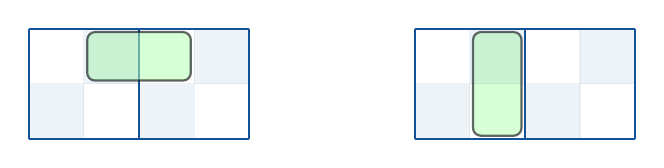
\begin{tikzpicture}[tableau, scale = .7]
          \gridLines{1}{2}
          \horizontalDominoRS{1}{2}{}
          \fixedSquaresForGrid{1}{2}

          \gridLinesShift{1}{2}{7}
          \verticalDominoRSShift{1}{2}{ }{7}
          \fixedSquaresForGridShift{1}{2}{7}
        \end{tikzpicture}
      \end{figure}
      goes to
      \begin{figure}[H]
        \centering
        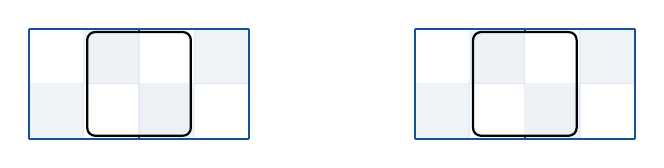
\begin{tikzpicture}[tableau, scale = .7]
          \gridLines{1}{2}
          \emptyBox{1}{2}
          \fixedSquaresForGrid{1}{2}

          \gridLinesShift{1}{2}{7}
          \emptyBoxShift{1}{2}{7}
          \fixedSquaresForGridShift{1}{2}{7}
        \end{tikzpicture}
      \end{figure}
      \begin{figure}[H]
        % 1_2
        \centering
        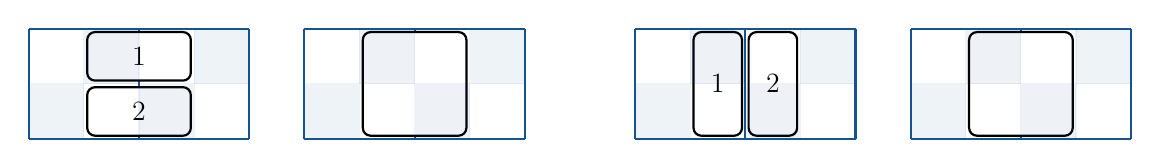
\begin{tikzpicture}[tableau, scale=.7]\gridLines{1}{2}\horizontalDomino{1}{2}{1}\horizontalDomino{2}{2}{2}\fixedSquaresForGrid{1}{2}\gridLinesShift{1}{2}{5}\emptyBoxShift{1}{2}{5}\fixedSquaresForGridShift{1}{2}{5}\gridLinesShift{1}{2}{11}\verticalDominoShift{1}{2}{1}{11}\verticalDominoShift{1}{3}{2}{11}\fixedSquaresForGridShift{1}{2}{11}\gridLinesShift{1}{2}{16}\emptyBoxShift{1}{2}{16}\fixedSquaresForGridShiftAlt{1}{2}{16}\end{tikzpicture}
      \end{figure}
      Here is a more complicated example.
      \begin{figure}[H]
        \centering
        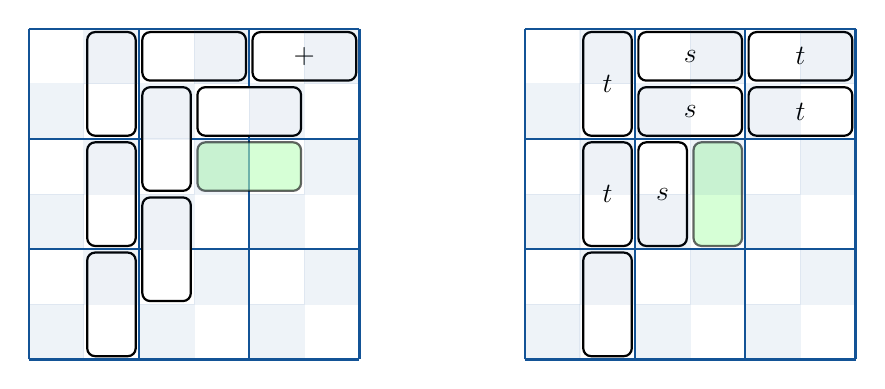
\begin{tikzpicture}[tableau, scale = .7]
          \gridLines{3}{3}
          \verticalDomino{1}{2}{ }
          \horizontalDomino{1}{3}{ }
          \horizontalDomino{1}{5}{+}
          \verticalDomino{3}{2}{ }
          \verticalDomino{2}{3}{ }
          \horizontalDomino{2}{4}{ }
          \horizontalDominoRS{3}{4}{}
          \verticalDomino{4}{3}{ }
          \verticalDomino{5}{2}{}
          \fixedSquaresForGrid{3}{3}

          \gridLinesShift{3}{3}{9}
          \verticalDominoShift{1}{2}{t}{9}
          \horizontalDominoShift{1}{3}{s}{9}
          \horizontalDominoShift{1}{5}{t}{9}
          \horizontalDominoShift{2}{5}{t}{9}
          \verticalDominoShift{3}{2}{t}{9}
          \horizontalDominoShift{2}{3}{s}{9}
          \verticalDominoShift{5}{2}{ }{9}
          \verticalDominoShift{3}{3}{s}{9}
          \verticalDominoRSShift{3}{4}{ }{9}
          \fixedSquaresForGridShift{3}{3}{9}
        \end{tikzpicture}
      \end{figure}
      goes to
      \begin{figure}[H]
        \centering
        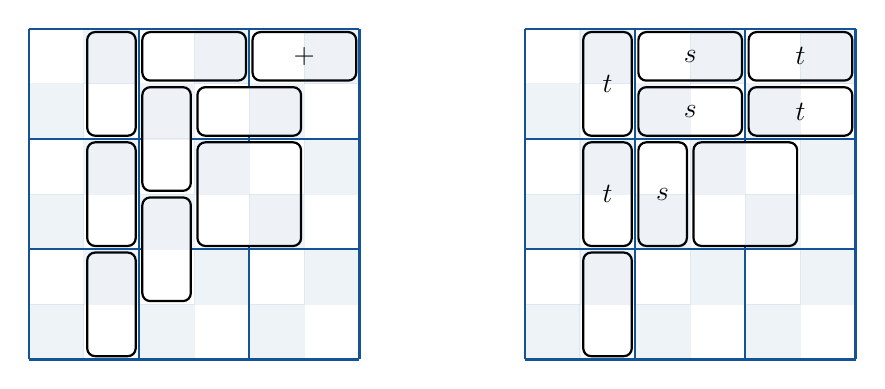
\begin{tikzpicture}[tableau, scale = .7]
          \gridLines{3}{3}
          \verticalDomino{1}{2}{ }
          \horizontalDomino{1}{3}{ }
          \horizontalDomino{1}{5}{+}
          \verticalDomino{3}{2}{ }
          \verticalDomino{2}{3}{ }
          \horizontalDomino{2}{4}{ }
          \emptyBox{3}{4}
          \verticalDomino{4}{3}{ }
          \verticalDomino{5}{2}{}
          \fixedSquaresForGrid{3}{3}

          \gridLinesShift{3}{3}{9}
          \verticalDominoShift{1}{2}{t}{9}
          \horizontalDominoShift{1}{3}{s}{9}
          \horizontalDominoShift{1}{5}{t}{9}
          \horizontalDominoShift{2}{5}{t}{9}
          \verticalDominoShift{3}{2}{t}{9}
          \horizontalDominoShift{2}{3}{s}{9}
          \verticalDominoShift{5}{2}{ }{9}
          \verticalDominoShift{3}{3}{s}{9}
          \emptyBoxShift{3}{4}{9}
          \fixedSquaresForGridShift{3}{3}{9}
        \end{tikzpicture}
      \end{figure}
      goes to
      \begin{figure}[H]
        \centering
        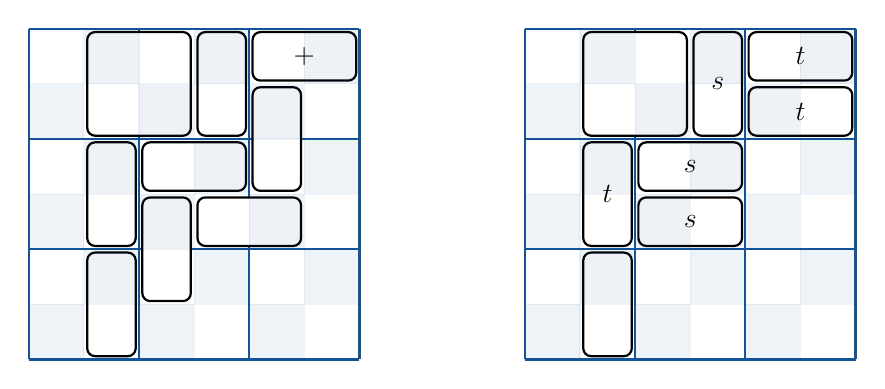
\begin{tikzpicture}[tableau, scale = .7]
          \gridLines{3}{3}
          \emptyBox{1}{2}
          \verticalDomino{1}{4}{}
          \horizontalDomino{1}{5}{+}
          \verticalDomino{2}{5}{}
          \horizontalDomino{3}{3}{}
          \horizontalDomino{4}{4}{}
          \verticalDomino{3}{2}{}
          \verticalDomino{4}{3}{ }
          \verticalDomino{5}{2}{}
          \fixedSquaresForGrid{3}{3}

          \gridLinesShift{3}{3}{9}
          \emptyBoxShift{1}{2}{9}
          \verticalDominoShift{1}{4}{s}{9}
          \horizontalDominoShift{1}{5}{t}{9}
          \horizontalDominoShift{2}{5}{t}{9}
          \verticalDominoShift{3}{2}{t}{9}
          \horizontalDominoShift{3}{3}{s}{9}
          \verticalDominoShift{5}{2}{}{9}
          \horizontalDominoShift{4}{3}{s}{9}
          \fixedSquaresForGridShift{3}{3}{9}
        \end{tikzpicture}
      \end{figure}
      \begin{figure}[H]
        % 1t 2- 3s 4s 5t 6t 8+ 9+ 7_10
        \centering
        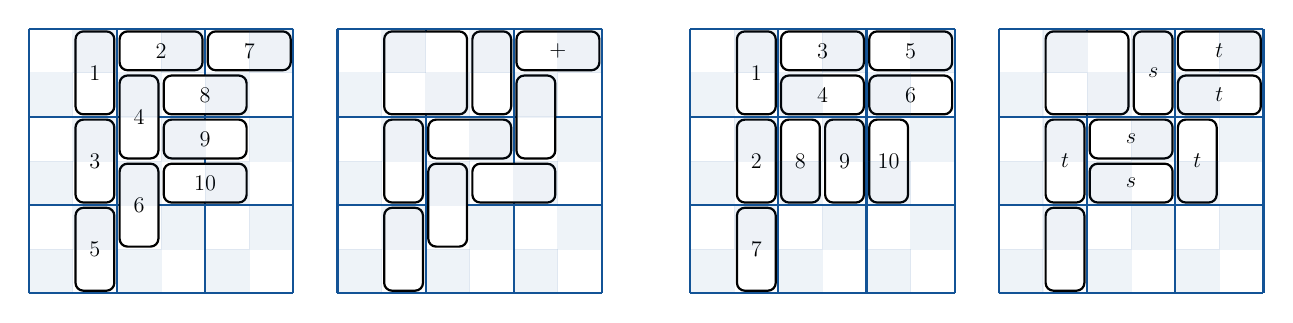
\begin{tikzpicture}[tableau, scale=.56]\gridLines{3}{3}\verticalDomino{1}{2}{1}\horizontalDomino{1}{3}{2}\verticalDomino{3}{2}{3}\verticalDomino{2}{3}{4}\verticalDomino{5}{2}{5}\verticalDomino{4}{3}{6}\horizontalDomino{1}{5}{7}\horizontalDomino{2}{4}{8}\horizontalDomino{3}{4}{9}\horizontalDomino{4}{4}{10}\fixedSquaresForGrid{3}{3}\gridLinesShift{3}{3}{7}\verticalDominoShift{1}{4}{}{7}\verticalDominoShift{3}{2}{}{7}\verticalDominoShift{5}{2}{}{7}\verticalDominoShift{4}{3}{}{7}\horizontalDominoShift{1}{5}{+}{7}\verticalDominoShift{2}{5}{}{7}\horizontalDominoShift{3}{3}{}{7}\horizontalDominoShift{4}{4}{}{7}\emptyBoxShift{1}{2}{7}\fixedSquaresForGridShift{3}{3}{7}\gridLinesShift{3}{3}{15}\verticalDominoShift{1}{2}{1}{15}\verticalDominoShift{3}{2}{2}{15}\horizontalDominoShift{1}{3}{3}{15}\horizontalDominoShift{2}{3}{4}{15}\horizontalDominoShift{1}{5}{5}{15}\horizontalDominoShift{2}{5}{6}{15}\verticalDominoShift{5}{2}{7}{15}\verticalDominoShift{3}{3}{8}{15}\verticalDominoShift{3}{4}{9}{15}\verticalDominoShift{3}{5}{10}{15}\fixedSquaresForGridShift{3}{3}{15}\gridLinesShift{3}{3}{22}\verticalDominoShift{3}{2}{t}{22}\verticalDominoShift{1}{4}{s}{22}\horizontalDominoShift{1}{5}{t}{22}\horizontalDominoShift{2}{5}{t}{22}\verticalDominoShift{5}{2}{}{22}\horizontalDominoShift{4}{3}{s}{22}\horizontalDominoShift{3}{3}{s}{22}\verticalDominoShift{3}{5}{t}{22}\emptyBoxShift{1}{2}{22}\fixedSquaresForGridShiftAlt{3}{3}{22}\end{tikzpicture}
      \end{figure}
      \item Here the next row has a shorter length.
      We'll use the new domino to contract an unboxed cycle.

      Basically, there are two cases for this insertion.
      On the one hand, there may be a sign in the vertical domino to the left.
      In that case, we give the new domino the opposite sign.
      This is compatible with the signs already in
      the cycle.
      So, we just add the domino, giving it the opposite sign to the one on the left, box things up, and then call \texttt{addNumberSign()} with the same sign as on the left.
      \begin{figure}[H]
        \centering
        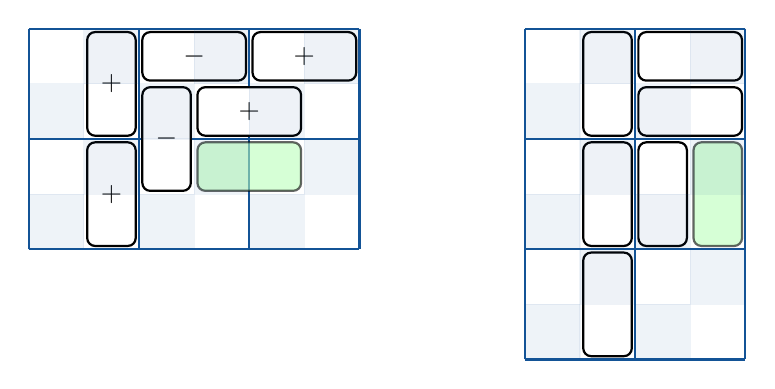
\begin{tikzpicture}[tableau, scale = .7]
          \gridLines{2}{3}
          \verticalDomino{1}{2}{+}
          \horizontalDomino{1}{3}{-}
          \horizontalDomino{1}{5}{+}
          \verticalDomino{3}{2}{+}
          \verticalDomino{2}{3}{-}
          \horizontalDomino{2}{4}{+}
          \horizontalDominoRS{3}{4}{}
          \fixedSquaresForGrid{2}{3}

          \gridLinesShift{3}{2}{9}
          \verticalDominoShift{1}{2}{}{9}
          \horizontalDominoShift{1}{3}{}{9}
          \verticalDominoShift{3}{2}{}{9}
          \horizontalDominoShift{2}{3}{}{9}
          \verticalDominoShift{5}{2}{ }{9}
          \verticalDominoShift{3}{3}{}{9}
          \verticalDominoRSShift{3}{4}{ }{9}
          \fixedSquaresForGridShift{3}{2}{9}
        \end{tikzpicture}
      \end{figure}
      goes to
      \begin{figure}[H]
        \centering
        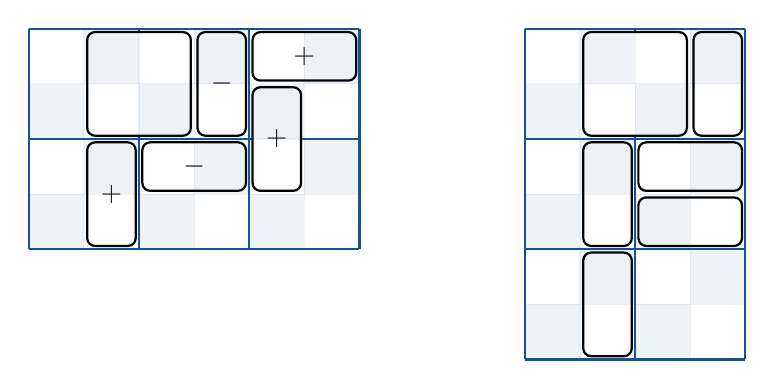
\begin{tikzpicture}[tableau, scale = .7]
          \gridLines{2}{3}
          \emptyBox{1}{2}
          \verticalDomino{1}{4}{-}
          \horizontalDomino{1}{5}{+}
          \verticalDomino{3}{2}{+}
          \verticalDomino{2}{5}{+}
          \horizontalDomino{3}{3}{-}
          \fixedSquaresForGrid{2}{3}

          \gridLinesShift{3}{2}{9}
          \emptyBoxShift{1}{2}{9}
          \verticalDominoShift{1}{4}{}{9}
          \verticalDominoShift{3}{2}{}{9}
          \verticalDominoShift{5}{2}{ }{9}
          \horizontalDominoShift{4}{3}{}{9}
          \horizontalDominoShift{3}{3}{ }{9}
          \fixedSquaresForGridShift{3}{2}{9}
        \end{tikzpicture}
      \end{figure}
      \begin{figure}[H]
        % 1+ 2- 3_-4 6+ 7+ 5_8
        \centering
        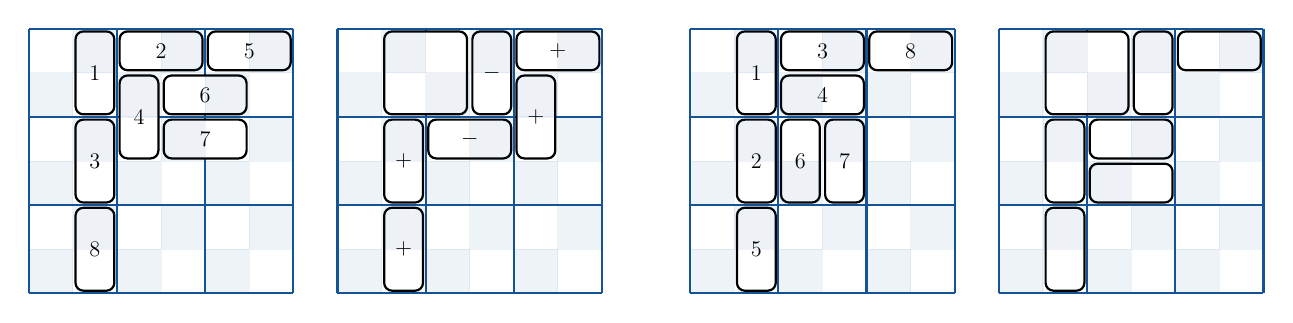
\begin{tikzpicture}[tableau, scale=.56]\gridLines{3}{3}\verticalDomino{1}{2}{1}\horizontalDomino{1}{3}{2}\verticalDomino{3}{2}{3}\verticalDomino{2}{3}{4}\horizontalDomino{1}{5}{5}\horizontalDomino{2}{4}{6}\horizontalDomino{3}{4}{7}\verticalDomino{5}{2}{8}\fixedSquaresForGrid{3}{3}\gridLinesShift{3}{3}{7}\verticalDominoShift{1}{4}{-}{7}\verticalDominoShift{3}{2}{+}{7}\horizontalDominoShift{1}{5}{+}{7}\verticalDominoShift{2}{5}{+}{7}\horizontalDominoShift{3}{3}{-}{7}\emptyBoxShift{1}{2}{7}\verticalDominoShift{5}{2}{+}{7}\fixedSquaresForGridShift{3}{3}{7}\gridLinesShift{3}{3}{15}\verticalDominoShift{1}{2}{1}{15}\verticalDominoShift{3}{2}{2}{15}\horizontalDominoShift{1}{3}{3}{15}\horizontalDominoShift{2}{3}{4}{15}\verticalDominoShift{5}{2}{5}{15}\verticalDominoShift{3}{3}{6}{15}\verticalDominoShift{3}{4}{7}{15}\horizontalDominoShift{1}{5}{8}{15}\fixedSquaresForGridShift{3}{3}{15}\gridLinesShift{3}{3}{22}\verticalDominoShift{3}{2}{}{22}\verticalDominoShift{1}{4}{}{22}\verticalDominoShift{5}{2}{}{22}\horizontalDominoShift{4}{3}{}{22}\horizontalDominoShift{3}{3}{}{22}\emptyBoxShift{1}{2}{22}\horizontalDominoShift{1}{5}{}{22}\fixedSquaresForGridShiftAlt{3}{3}{22}\end{tikzpicture}
      \end{figure}

      On the other hand, it may be that the domino to the left is blank.
      Now, note, the domino to the left is a cycle bottom.
      So, it follows that even if the left domino is horizontal, there is effectively no sign at that level.
      The only possible signed domino in that row would be a vertical domino which we can move down if necessary by calling \texttt{makeSpaceFor()}, which we do.
      (Any other sign would have already moved to the left domino, since any sign can go in a cycle bottom.)
      In addition, once we add a domino here, with either sign, the next domino will be able to add at the next row, and both signs will be blanked in that process, leaving this cycle with the same signs which it started with.
      So, that's what we expect to see, and what we see in the example below.

      So, for this step, if there is no sign in the left domino, we just choose the sign to add here for convenience, so that putting it in the cycle bottom doesn't move the cycle.
      So, we choose a compatible sign.
      To do that, we look at the top domino.
      If it has a sign, we choose its sign.
      If not, we look at the cycle top.
      If it has a sign, we use the function \texttt{getExpectedSign()} to choose a sign for the newly-added domino.
      If not, we choose a sign arbitrarily.
      In any case, once we've chosen the sign, we call \texttt{putSignInCycleBottom()}.

      Here is an example.
      \begin{figure}[H]
        \centering
        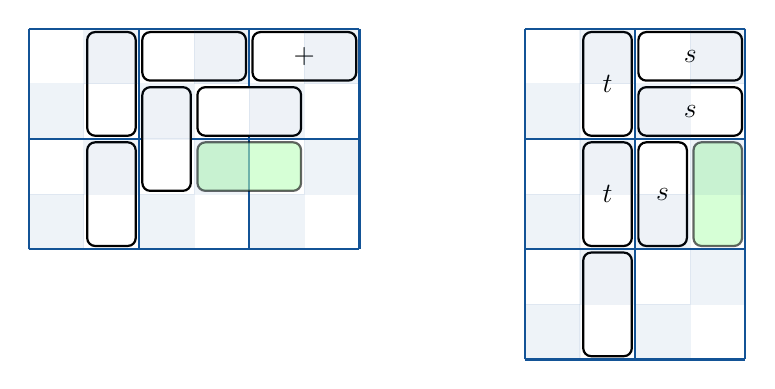
\begin{tikzpicture}[tableau, scale = .7]
          \gridLines{2}{3}
          \verticalDomino{1}{2}{ }
          \horizontalDomino{1}{3}{ }
          \horizontalDomino{1}{5}{+}
          \verticalDomino{3}{2}{ }
          \verticalDomino{2}{3}{ }
          \horizontalDomino{2}{4}{ }
          \horizontalDominoRS{3}{4}{}
          \fixedSquaresForGrid{2}{3}

          \gridLinesShift{3}{2}{9}
          \verticalDominoShift{1}{2}{t}{9}
          \horizontalDominoShift{1}{3}{s}{9}
          \verticalDominoShift{3}{2}{t}{9}
          \horizontalDominoShift{2}{3}{s}{9}
          \verticalDominoShift{5}{2}{ }{9}
          \verticalDominoShift{3}{3}{s}{9}
          \verticalDominoRSShift{3}{4}{ }{9}
          \fixedSquaresForGridShift{3}{2}{9}
        \end{tikzpicture}
      \end{figure}
      goes to
      \begin{figure}[H]
        \centering
        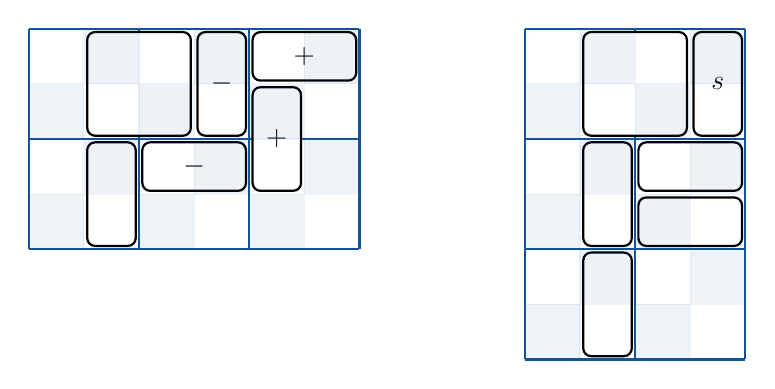
\begin{tikzpicture}[tableau, scale = .7]
          \gridLines{2}{3}
          \emptyBox{1}{2}
          \verticalDomino{1}{4}{-}
          \horizontalDomino{1}{5}{+}
          \verticalDomino{3}{2}{ }
          \verticalDomino{2}{5}{+}
          \horizontalDomino{3}{3}{-}
          \fixedSquaresForGrid{2}{3}

          \gridLinesShift{3}{2}{9}
          \emptyBoxShift{1}{2}{9}
          \verticalDominoShift{1}{4}{s}{9}
          \verticalDominoShift{3}{2}{}{9}
          \verticalDominoShift{5}{2}{ }{9}
          \horizontalDominoShift{4}{3}{}{9}
          \horizontalDominoShift{3}{3}{ }{9}
          \fixedSquaresForGridShift{3}{2}{9}
        \end{tikzpicture}
      \end{figure}
      \begin{figure}[H]
        % 1t 2- 3s 4s 6+ 7+ 5_8
        \centering
        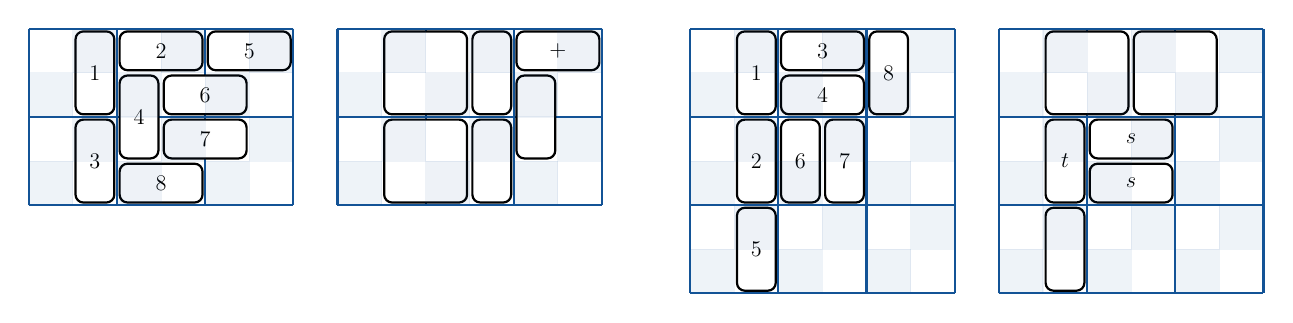
\begin{tikzpicture}[tableau, scale=.56]\gridLines{2}{3}\verticalDomino{1}{2}{1}\horizontalDomino{1}{3}{2}\verticalDomino{3}{2}{3}\verticalDomino{2}{3}{4}\horizontalDomino{1}{5}{5}\horizontalDomino{2}{4}{6}\horizontalDomino{3}{4}{7}\horizontalDomino{4}{3}{8}\fixedSquaresForGrid{2}{3}\gridLinesShift{2}{3}{7}\verticalDominoShift{1}{4}{}{7}\horizontalDominoShift{1}{5}{+}{7}\verticalDominoShift{2}{5}{}{7}\verticalDominoShift{3}{4}{}{7}\emptyBoxShift{1}{2}{7}\emptyBoxShift{3}{2}{7}\fixedSquaresForGridShift{2}{3}{7}\gridLinesShift{3}{3}{15}\verticalDominoShift{1}{2}{1}{15}\verticalDominoShift{3}{2}{2}{15}\horizontalDominoShift{1}{3}{3}{15}\horizontalDominoShift{2}{3}{4}{15}\verticalDominoShift{5}{2}{5}{15}\verticalDominoShift{3}{3}{6}{15}\verticalDominoShift{3}{4}{7}{15}\verticalDominoShift{1}{5}{8}{15}\fixedSquaresForGridShift{3}{3}{15}\gridLinesShift{3}{3}{22}\verticalDominoShift{3}{2}{t}{22}\verticalDominoShift{5}{2}{}{22}\horizontalDominoShift{4}{3}{s}{22}\horizontalDominoShift{3}{3}{s}{22}\emptyBoxShift{1}{2}{22}\emptyBoxShift{1}{4}{22}\fixedSquaresForGridShiftAlt{3}{3}{22}\end{tikzpicture}
      \end{figure}
    \end{itemize}

    \item Here $gpos$ and $dgpos$ are both $Y$, and both \pos\ and \dpos\ are vertical.
    This is an exceptional case.
    We make a box here, with both dominoes.
    Note, it's a little pecular that both positions come out vertical.
    This may need some discussion.
    In the example, one can see the issue that the dual number tableau is not just transposed but also cycled through.
    Probably, something needs proving here.
    \begin{figure}[H]
      \centering
      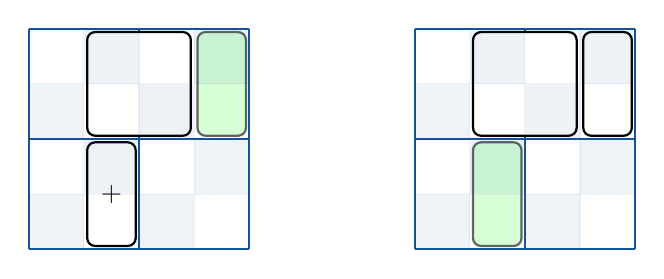
\begin{tikzpicture}[tableau, scale = .7]
        \gridLines{2}{2}
        \emptyBox{1}{2}
        \verticalDomino{3}{2}{+}
        \verticalDominoRS{1}{4}{}
        \fixedSquaresForGrid{2}{2}

        \gridLinesShift{2}{2}{7}
        \emptyBoxShift{1}{2}{7}
        \verticalDominoShift{1}{4}{}{7}
        \verticalDominoRSShift{3}{2}{}{7}
        \fixedSquaresForGridShift{2}{2}{7}
      \end{tikzpicture}
    \end{figure}
    goes to
    \begin{figure}[H]
      \centering
      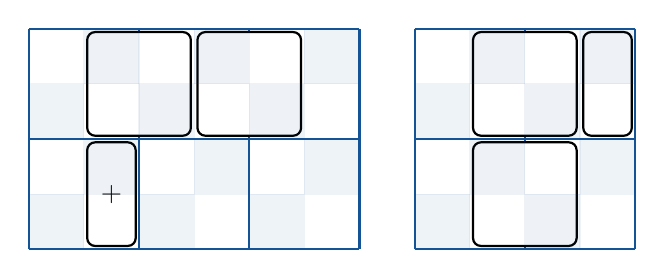
\begin{tikzpicture}[tableau, scale = .7]
        \gridLines{2}{3}
        \emptyBox{1}{2}
        \verticalDomino{3}{2}{+}
        \emptyBox{1}{4}
        \fixedSquaresForGrid{2}{3}

        \gridLinesShift{2}{2}{7}
        \emptyBoxShift{1}{2}{7}
        \verticalDominoShift{1}{4}{}{7}
        \emptyBoxShift{3}{2}{7}
        \fixedSquaresForGridShift{2}{2}{7}
      \end{tikzpicture}
    \end{figure}
    \begin{figure}[H]
      % 1+ 2_-4
      \centering
      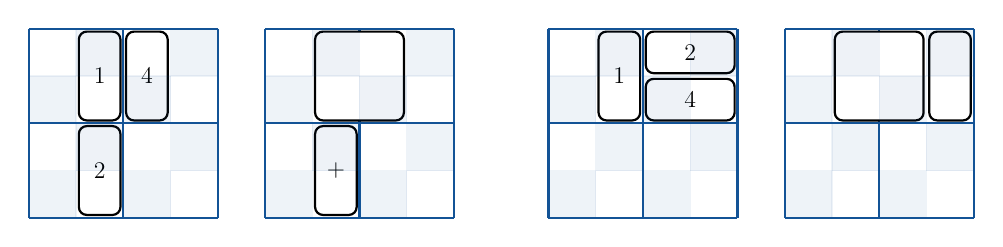
\begin{tikzpicture}[tableau, scale=.6]\gridLines{2}{2}\verticalDomino{1}{2}{1}\verticalDomino{3}{2}{2}\verticalDomino{1}{3}{4}\fixedSquaresForGrid{2}{2}\gridLinesShift{2}{2}{5}\verticalDominoShift{3}{2}{+}{5}\emptyBoxShift{1}{2}{5}\fixedSquaresForGridShift{2}{2}{5}
      \gridLinesShift{2}{2}{11}\verticalDominoShift{1}{2}{1}{11}\horizontalDominoShift{1}{3}{2}{11}\horizontalDominoShift{2}{3}{4}{11}\fixedSquaresForGridShift{2}{2}{11}\gridLinesShift{2}{2}{16}\verticalDominoShift{1}{4}{}{16}\emptyBoxShift{1}{2}{16}\fixedSquaresForGridShiftAlt{2}{2}{16}\end{tikzpicture}
    \end{figure}
    goes to
    \begin{figure}[H]
      % 1+ 2_-4 3_5
      \centering
      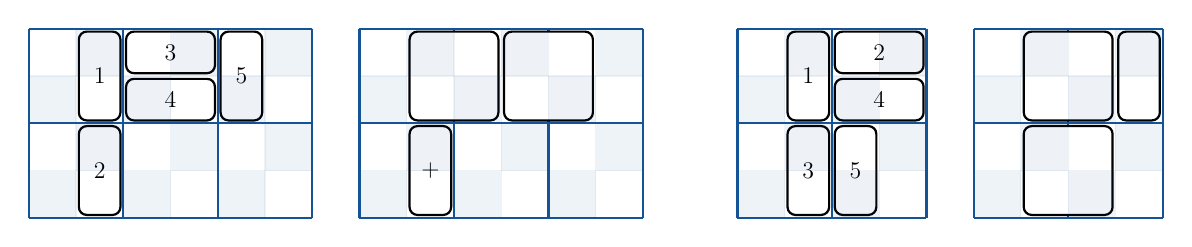
\begin{tikzpicture}[tableau, scale=.6]\gridLines{2}{3}\verticalDomino{1}{2}{1}\verticalDomino{3}{2}{2}\horizontalDomino{1}{3}{3}\horizontalDomino{2}{3}{4}\verticalDomino{1}{5}{5}\fixedSquaresForGrid{2}{3}\gridLinesShift{2}{3}{7}\verticalDominoShift{3}{2}{+}{7}\emptyBoxShift{1}{2}{7}\emptyBoxShift{1}{4}{7}\fixedSquaresForGridShift{2}{3}{7}\gridLinesShift{2}{2}{15}\verticalDominoShift{1}{2}{1}{15}\horizontalDominoShift{1}{3}{2}{15}\verticalDominoShift{3}{2}{3}{15}\horizontalDominoShift{2}{3}{4}{15}\verticalDominoShift{3}{3}{5}{15}\fixedSquaresForGridShift{2}{2}{15}\gridLinesShift{2}{2}{20}\verticalDominoShift{1}{4}{}{20}\emptyBoxShift{1}{2}{20}\emptyBoxShift{3}{2}{20}\fixedSquaresForGridShiftAlt{2}{2}{20}\end{tikzpicture}
    \end{figure}

    \item Here $gpos$ and $dgpos$ are both $X$, and both \pos\ and \dpos\ are vertical.
    As in the previous case, this has to do with being cycled through.
    On one side the new position will be next to a vertical domino with a sign in it (which we will assume to be plus), on the other side enxt to a blank domino.
    We will box up the new positions, and add a $+$ sign below the former $+$ sign domino.
    \begin{figure}[H]
      \centering
      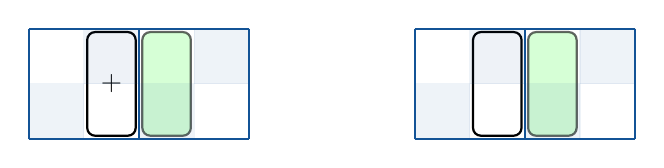
\begin{tikzpicture}[tableau, scale = .7]
        \gridLines{1}{2}
        \verticalDomino{1}{2}{+}
        \verticalDominoRS{1}{3}{}
        \fixedSquaresForGrid{1}{2}

        \gridLinesShift{1}{2}{7}
        \verticalDominoShift{1}{2}{}{7}
        \verticalDominoRSShift{1}{3}{}{7}
        \fixedSquaresForGridShift{1}{2}{7}
      \end{tikzpicture}
    \end{figure}
    goes to
    \begin{figure}[H]
      \centering
      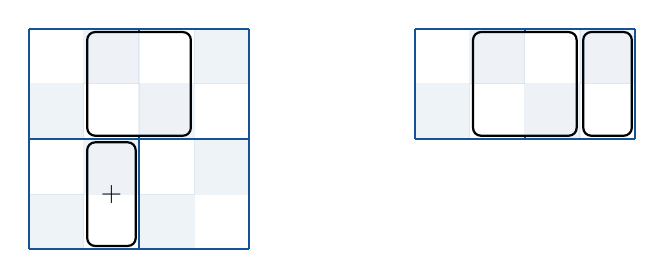
\begin{tikzpicture}[tableau, scale = .7]
        \gridLines{2}{2}
        \emptyBox{1}{2}
        \verticalDomino{3}{2}{+}
        \fixedSquaresForGrid{2}{2}

        \gridLinesShift{1}{2}{7}
        \emptyBoxShift{1}{2}{7}
        \verticalDominoShift{1}{4}{}{7}
        \fixedSquaresForGridShift{1}{2}{7}
      \end{tikzpicture}
    \end{figure}
    \begin{figure}[H]
      % 2+
      \centering
      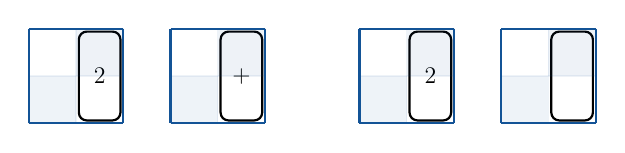
\begin{tikzpicture}[tableau, scale=.6]\gridLines{1}{1}\verticalDomino{1}{2}{2}\fixedSquaresForGrid{1}{1}\gridLinesShift{1}{1}{3}\verticalDominoShift{1}{2}{+}{3}\fixedSquaresForGridShift{1}{1}{3}\gridLinesShift{1}{1}{7}\verticalDominoShift{1}{2}{2}{7}\fixedSquaresForGridShift{1}{1}{7}\gridLinesShift{1}{1}{10}\verticalDominoShift{1}{2}{}{10}\fixedSquaresForGridShiftAlt{1}{1}{10}\end{tikzpicture}
    \end{figure}
    goes to
    \begin{figure}[H]
      % 2+ 1_3
      \centering
      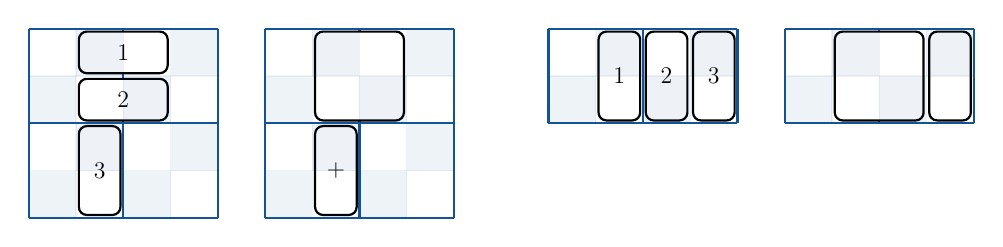
\begin{tikzpicture}[tableau, scale=.6]\gridLines{2}{2}\horizontalDomino{1}{2}{1}\horizontalDomino{2}{2}{2}\verticalDomino{3}{2}{3}\fixedSquaresForGrid{2}{2}\gridLinesShift{2}{2}{5}\emptyBoxShift{1}{2}{5}\verticalDominoShift{3}{2}{+}{5}\fixedSquaresForGridShift{2}{2}{5}\gridLinesShift{1}{2}{11}\verticalDominoShift{1}{2}{1}{11}\verticalDominoShift{1}{3}{2}{11}\verticalDominoShift{1}{4}{3}{11}\fixedSquaresForGridShift{1}{2}{11}\gridLinesShift{1}{2}{16}\emptyBoxShift{1}{2}{16}\verticalDominoShift{1}{4}{}{16}\fixedSquaresForGridShiftAlt{1}{2}{16}\end{tikzpicture}
    \end{figure}

    \item Here $gpos = X$ and \pos\ is horizontal.
    There are a number of cases.
    We split on how the cycle structures of the tableaux are changed by the addition of the dominoes.
    (Note, I wrote about using \texttt{makeSpaceFor()}, but actually, I didn't change the code yet to use that function.)
    \begin{itemize}
      \item Here the added domino extends a Type I cycle.
      If there's a sign in the domino directly to the left, we put the opposite sign into the newly-added domino; otherwise we choose an arbitrary sign.
      In the case where we choose an arbitrary sign, that choice will be blanked once the next domino is added at the row after.
      For now, we make sure we can place the arbitrary sign here by calling \texttt{makeSpaceFor()}.
      Note, there is no need to avoid the effort of moving a sign down by making a sign choice which is compatible with whatever sign is at the end of this row.
      If there is a sign at the end of the row, it would have to move down anyway when we come to add the second domino of the pair.

      Here are three examples.
      \begin{figure}[H]
        \centering
        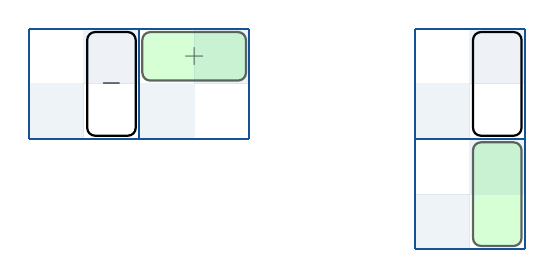
\begin{tikzpicture}[tableau, scale = .7]
          \gridLines{1}{2}
          \verticalDomino{1}{2}{-}
          \horizontalDominoRS{1}{3}{+}
          \fixedSquaresForGrid{1}{2}

          \gridLinesShift{2}{1}{7}
          \verticalDominoShift{1}{2}{}{7}
          \verticalDominoRSShift{3}{2}{}{7}
          \fixedSquaresForGridShift{2}{1}{7}
        \end{tikzpicture}
      \end{figure}
      \begin{figure}[H]
        % 1-
        \centering
        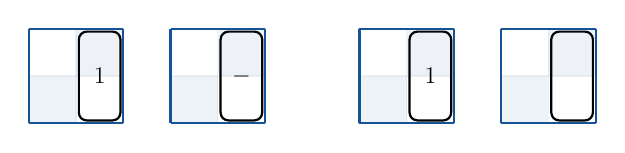
\begin{tikzpicture}[tableau, scale=.6]\gridLines{1}{1}\verticalDomino{1}{2}{1}\fixedSquaresForGrid{1}{1}\gridLinesShift{1}{1}{3}\verticalDominoShift{1}{2}{-}{3}\fixedSquaresForGridShift{1}{1}{3}\gridLinesShift{1}{1}{7}\verticalDominoShift{1}{2}{1}{7}\fixedSquaresForGridShift{1}{1}{7}\gridLinesShift{1}{1}{10}\verticalDominoShift{1}{2}{}{10}\fixedSquaresForGridShiftAlt{1}{1}{10}\end{tikzpicture}
      \end{figure}
      goes to
      \begin{figure}[H]
        % 1- 2_3
        \centering
        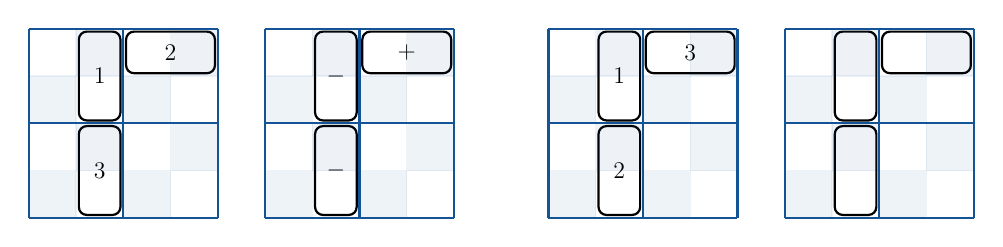
\begin{tikzpicture}[tableau, scale=.6]\gridLines{2}{2}\verticalDomino{1}{2}{1}\horizontalDomino{1}{3}{2}\verticalDomino{3}{2}{3}\fixedSquaresForGrid{2}{2}\gridLinesShift{2}{2}{5}\verticalDominoShift{1}{2}{-}{5}\horizontalDominoShift{1}{3}{+}{5}\verticalDominoShift{3}{2}{-}{5}\fixedSquaresForGridShift{2}{2}{5}\gridLinesShift{2}{2}{11}\verticalDominoShift{1}{2}{1}{11}\verticalDominoShift{3}{2}{2}{11}\horizontalDominoShift{1}{3}{3}{11}\fixedSquaresForGridShift{2}{2}{11}\gridLinesShift{2}{2}{16}\verticalDominoShift{1}{2}{}{16}\verticalDominoShift{3}{2}{}{16}\horizontalDominoShift{1}{3}{}{16}\fixedSquaresForGridShiftAlt{2}{2}{16}\end{tikzpicture}
      \end{figure}
      Next example:
      \begin{figure}[H]
        \centering
        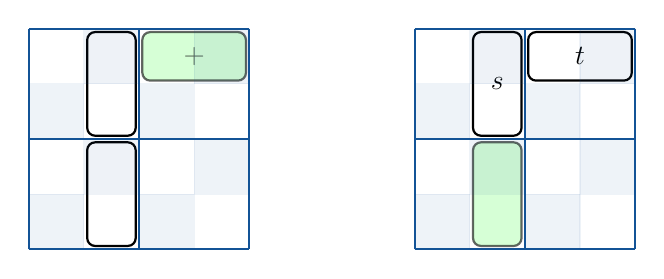
\begin{tikzpicture}[tableau, scale = .7]
          \gridLines{2}{2}
          \verticalDomino{1}{2}{}
          \horizontalDominoRS{1}{3}{+}
          \verticalDomino{3}{2}{}
          \fixedSquaresForGrid{2}{2}

          \gridLinesShift{2}{2}{7}
          \verticalDominoShift{1}{2}{s}{7}
          \horizontalDominoShift{1}{3}{t}{7}
          \verticalDominoRSShift{3}{2}{}{7}
          \fixedSquaresForGridShift{2}{2}{7}
        \end{tikzpicture}
      \end{figure}
      \begin{figure}[H]
        % 1s 2t
        \centering
        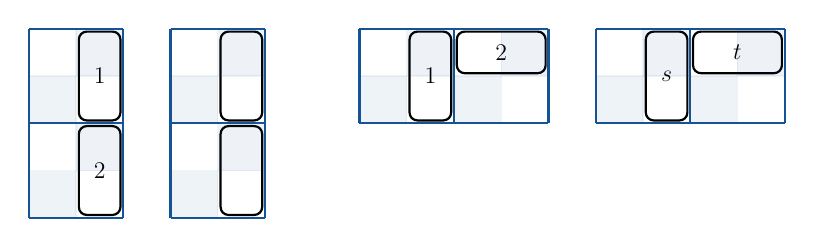
\begin{tikzpicture}[tableau, scale=.6]\gridLines{2}{1}\verticalDomino{1}{2}{1}\verticalDomino{3}{2}{2}\fixedSquaresForGrid{2}{1}\gridLinesShift{2}{1}{3}\verticalDominoShift{1}{2}{}{3}\verticalDominoShift{3}{2}{}{3}\fixedSquaresForGridShift{2}{1}{3}\gridLinesShift{1}{2}{7}\verticalDominoShift{1}{2}{1}{7}\horizontalDominoShift{1}{3}{2}{7}\fixedSquaresForGridShift{1}{2}{7}\gridLinesShift{1}{2}{12}\verticalDominoShift{1}{2}{s}{12}\horizontalDominoShift{1}{3}{t}{12}\fixedSquaresForGridShiftAlt{1}{2}{12}\end{tikzpicture}
      \end{figure}
      goes to
      \begin{figure}[H]
        % 1s 2t 3_4
        \centering
        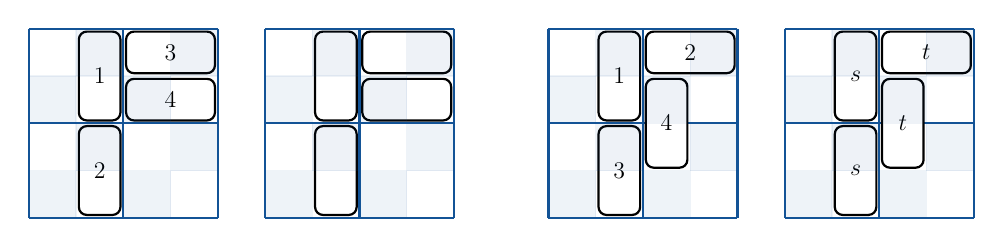
\begin{tikzpicture}[tableau, scale=.6]\gridLines{2}{2}\verticalDomino{1}{2}{1}\verticalDomino{3}{2}{2}\horizontalDomino{1}{3}{3}\horizontalDomino{2}{3}{4}\fixedSquaresForGrid{2}{2}\gridLinesShift{2}{2}{5}\verticalDominoShift{1}{2}{}{5}\verticalDominoShift{3}{2}{}{5}\horizontalDominoShift{1}{3}{}{5}\horizontalDominoShift{2}{3}{}{5}\fixedSquaresForGridShift{2}{2}{5}\gridLinesShift{2}{2}{11}\verticalDominoShift{1}{2}{1}{11}\horizontalDominoShift{1}{3}{2}{11}\verticalDominoShift{3}{2}{3}{11}\verticalDominoShift{2}{3}{4}{11}\fixedSquaresForGridShift{2}{2}{11}\gridLinesShift{2}{2}{16}\verticalDominoShift{1}{2}{s}{16}\horizontalDominoShift{1}{3}{t}{16}\verticalDominoShift{3}{2}{s}{16}\verticalDominoShift{2}{3}{t}{16}\fixedSquaresForGridShiftAlt{2}{2}{16}\end{tikzpicture}
      \end{figure}
      Third example:
      \begin{figure}[H]
        \centering
        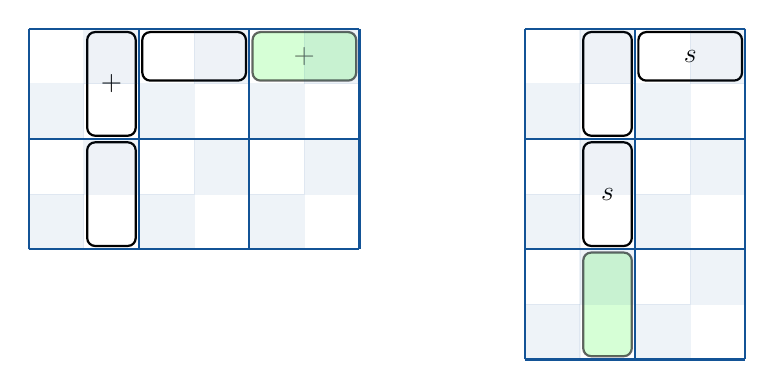
\begin{tikzpicture}[tableau, scale = .7]
          \gridLines{2}{3}
          \verticalDomino{1}{2}{+}
          \horizontalDomino{1}{3}{}
          \horizontalDominoRS{1}{5}{+}
          \verticalDomino{3}{2}{}
          \fixedSquaresForGrid{2}{3}

          \gridLinesShift{3}{2}{9}
          \verticalDominoShift{1}{2}{}{9}
          \horizontalDominoShift{1}{3}{s}{9}
          \verticalDominoShift{3}{2}{s}{9}
          \verticalDominoRSShift{5}{2}{}{9}
          \fixedSquaresForGridShift{3}{2}{9}
        \end{tikzpicture}
      \end{figure}
      goes to (via \texttt{makeSpaceFor()})
      \begin{figure}[H]
        \centering
        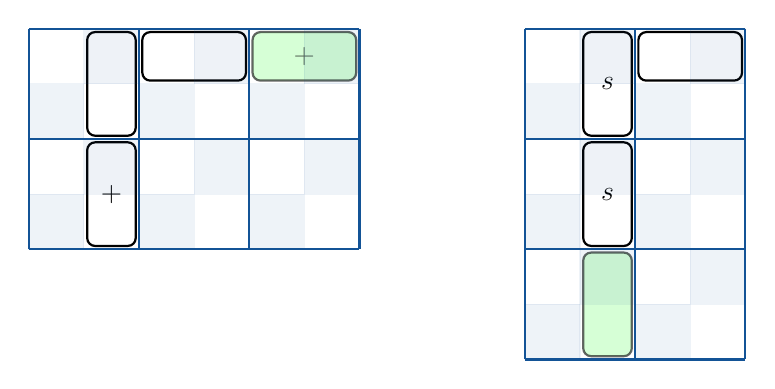
\begin{tikzpicture}[tableau, scale = .7]
          \gridLines{2}{3}
          \verticalDomino{1}{2}{}
          \horizontalDomino{1}{3}{}
          \horizontalDominoRS{1}{5}{+}
          \verticalDomino{3}{2}{+}
          \fixedSquaresForGrid{2}{3}

          \gridLinesShift{3}{2}{9}
          \verticalDominoShift{1}{2}{s}{9}
          \horizontalDominoShift{1}{3}{}{9}
          \verticalDominoShift{3}{2}{s}{9}
          \verticalDominoRSShift{5}{2}{}{9}
          \fixedSquaresForGridShift{3}{2}{9}
        \end{tikzpicture}
      \end{figure}
      \begin{figure}[H]
        % 1s 2+ 4s
        \centering
        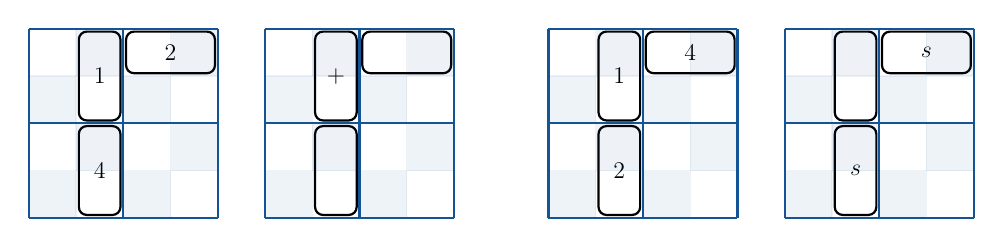
\begin{tikzpicture}[tableau, scale=.6]\gridLines{2}{2}\verticalDomino{1}{2}{1}\horizontalDomino{1}{3}{2}\verticalDomino{3}{2}{4}\fixedSquaresForGrid{2}{2}\gridLinesShift{2}{2}{5}\verticalDominoShift{1}{2}{+}{5}\horizontalDominoShift{1}{3}{}{5}\verticalDominoShift{3}{2}{}{5}\fixedSquaresForGridShift{2}{2}{5}\gridLinesShift{2}{2}{11}\verticalDominoShift{1}{2}{1}{11}\verticalDominoShift{3}{2}{2}{11}\horizontalDominoShift{1}{3}{4}{11}\fixedSquaresForGridShift{2}{2}{11}\gridLinesShift{2}{2}{16}\verticalDominoShift{1}{2}{}{16}\verticalDominoShift{3}{2}{s}{16}\horizontalDominoShift{1}{3}{s}{16}\fixedSquaresForGridShiftAlt{2}{2}{16}\end{tikzpicture}
      \end{figure}
      goes to
      \begin{figure}[H]
        % 1s 2+ 4s 3_5
        \centering
        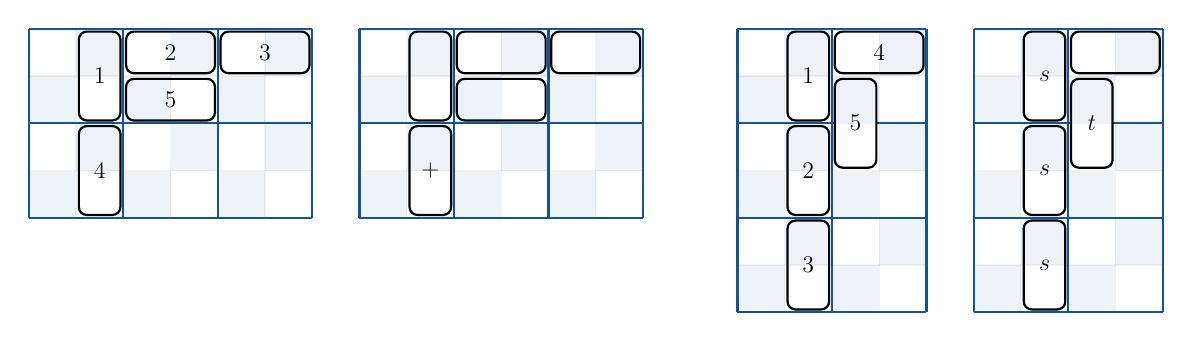
\begin{tikzpicture}[tableau, scale=.6]\gridLines{2}{3}\verticalDomino{1}{2}{1}\horizontalDomino{1}{3}{2}\horizontalDomino{1}{5}{3}\verticalDomino{3}{2}{4}\horizontalDomino{2}{3}{5}\fixedSquaresForGrid{2}{3}\gridLinesShift{2}{3}{7}\verticalDominoShift{1}{2}{}{7}\horizontalDominoShift{1}{3}{}{7}\verticalDominoShift{3}{2}{+}{7}\horizontalDominoShift{1}{5}{}{7}\horizontalDominoShift{2}{3}{}{7}\fixedSquaresForGridShift{2}{3}{7}\gridLinesShift{3}{2}{15}\verticalDominoShift{1}{2}{1}{15}\verticalDominoShift{3}{2}{2}{15}\verticalDominoShift{5}{2}{3}{15}\horizontalDominoShift{1}{3}{4}{15}\verticalDominoShift{2}{3}{5}{15}\fixedSquaresForGridShift{3}{2}{15}\gridLinesShift{3}{2}{20}\verticalDominoShift{1}{2}{s}{20}\verticalDominoShift{3}{2}{s}{20}\horizontalDominoShift{1}{3}{}{20}\verticalDominoShift{5}{2}{s}{20}\verticalDominoShift{2}{3}{t}{20}\fixedSquaresForGridShiftAlt{3}{2}{20}\end{tikzpicture}
      \end{figure}

      \item Here we are contracting a boxed Type II cycle.
      Again, if there is a sign to the left, we take the opposite sign to it.
      Also, again, if there is blank to the left, we don't care that much which sign we put here, since the sign will be blanked when the second domino is added.
      However, after we place the new domino and make a box, the new domino will be attached to the domino two rows above it.
      So, if the domino two rows above has a sign, we'll choose the same sign for the domino which we are adding.
      (Note, the side domino is the cycle bottom, whereas the above domino is a paired domino in the cycle.
      So, if they both have signs, they will have opposite signs.
      So, in that case, the two prescriptions have the same result.)
      If neither has a sign, we make an arbitrary choice.
      As above, if the side domino is blank, we call
      \texttt{makeSpaceFor()} before adding the domino.
      In all the cases, after we add the dominoes, we box them up.
      \begin{figure}[H]
        \centering
        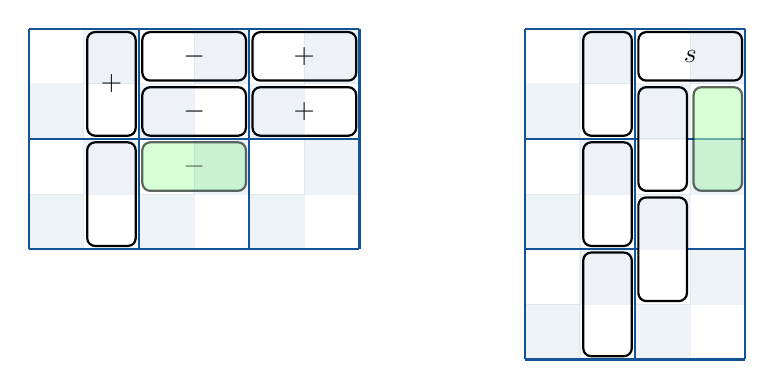
\begin{tikzpicture}[tableau, scale = .7]
          \gridLines{2}{3}
          \verticalDomino{1}{2}{+}
          \horizontalDomino{1}{3}{-}
          \horizontalDomino{1}{5}{+}
          \verticalDomino{3}{2}{ }
          \horizontalDomino{2}{3}{-}
          \horizontalDomino{2}{5}{+}
          \horizontalDominoRS{3}{3}{-}
          \fixedSquaresForGrid{2}{3}

          \gridLinesShift{3}{2}{9}
          \verticalDominoShift{1}{2}{}{9}
          \horizontalDominoShift{1}{3}{s}{9}
          \verticalDominoShift{3}{2}{}{9}
          \verticalDominoShift{2}{3}{}{9}
          \verticalDominoShift{5}{2}{ }{9}
          \verticalDominoShift{4}{3}{}{9}
          \verticalDominoRSShift{2}{4}{ }{9}
          \fixedSquaresForGridShift{3}{2}{9}
        \end{tikzpicture}
      \end{figure}
      goes to
      \begin{figure}[H]
        \centering
        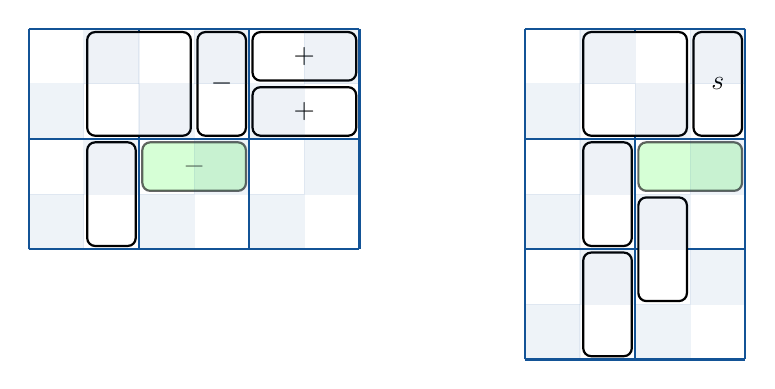
\begin{tikzpicture}[tableau, scale = .7]
          \gridLines{2}{3}
          \emptyBox{1}{2}
          \verticalDomino{1}{4}{-}
          \horizontalDomino{1}{5}{+}
          \verticalDomino{3}{2}{ }
          \horizontalDomino{2}{5}{+}
          \horizontalDominoRS{3}{3}{-}
          \fixedSquaresForGrid{2}{3}

          \gridLinesShift{3}{2}{9}
          \emptyBoxShift{1}{2}{9}
          \verticalDominoShift{1}{4}{s}{9}
          \verticalDominoShift{3}{2}{}{9}
          \verticalDominoShift{5}{2}{ }{9}
          \verticalDominoShift{4}{3}{}{9}
          \horizontalDominoRSShift{3}{3}{ }{9}
          \fixedSquaresForGridShift{3}{2}{9}
        \end{tikzpicture}
      \end{figure}
      \begin{figure}[H]
        % 1+ 2s 3- 4- 6+ 7+
        \centering
        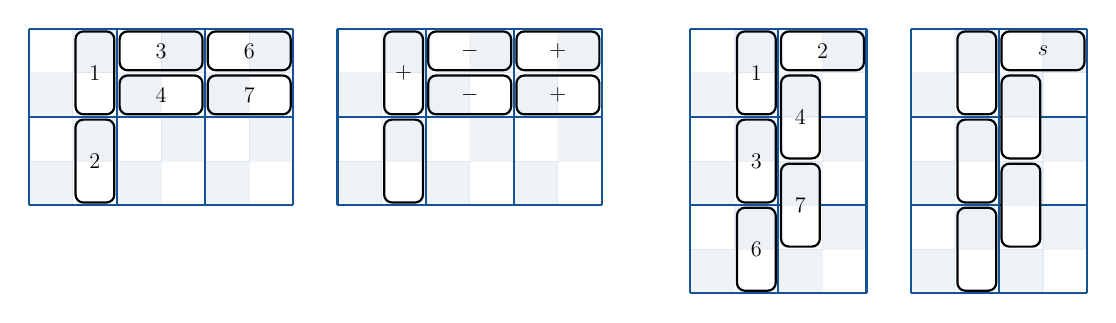
\begin{tikzpicture}[tableau, scale=.56]\gridLines{2}{3}\verticalDomino{1}{2}{1}\verticalDomino{3}{2}{2}\horizontalDomino{1}{3}{3}\horizontalDomino{2}{3}{4}\horizontalDomino{1}{5}{6}\horizontalDomino{2}{5}{7}\fixedSquaresForGrid{2}{3}\gridLinesShift{2}{3}{7}\verticalDominoShift{1}{2}{+}{7}\verticalDominoShift{3}{2}{}{7}\horizontalDominoShift{1}{3}{-}{7}\horizontalDominoShift{2}{3}{-}{7}\horizontalDominoShift{1}{5}{+}{7}\horizontalDominoShift{2}{5}{+}{7}\fixedSquaresForGridShift{2}{3}{7}\gridLinesShift{3}{2}{15}\verticalDominoShift{1}{2}{1}{15}\horizontalDominoShift{1}{3}{2}{15}\verticalDominoShift{3}{2}{3}{15}\verticalDominoShift{2}{3}{4}{15}\verticalDominoShift{5}{2}{6}{15}\verticalDominoShift{4}{3}{7}{15}\fixedSquaresForGridShift{3}{2}{15}\gridLinesShift{3}{2}{20}\verticalDominoShift{1}{2}{}{20}\horizontalDominoShift{1}{3}{s}{20}\verticalDominoShift{3}{2}{}{20}\verticalDominoShift{2}{3}{}{20}\verticalDominoShift{5}{2}{}{20}\verticalDominoShift{4}{3}{}{20}\fixedSquaresForGridShiftAlt{3}{2}{20}\end{tikzpicture}
      \end{figure}
      goes to
      \begin{figure}[H]
        % 1+ 2s 3- 4- 6+ 7+ 5_8
        \centering
        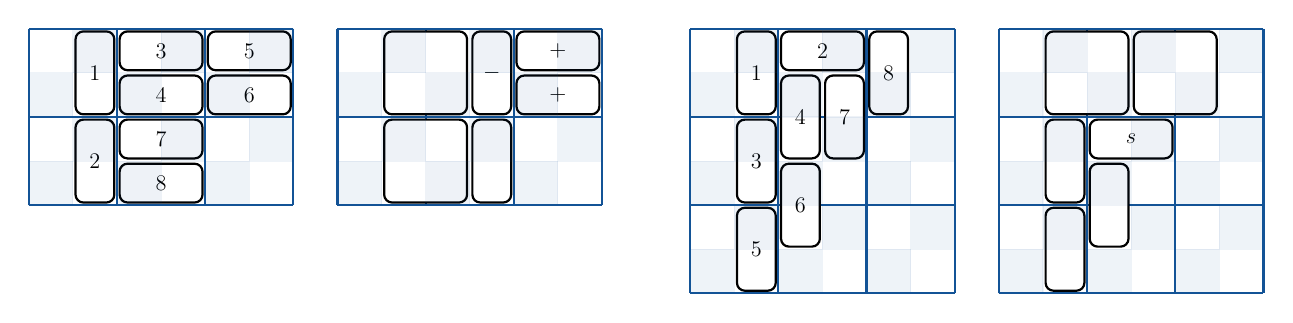
\begin{tikzpicture}[tableau, scale=.56]\gridLines{2}{3}\verticalDomino{1}{2}{1}\verticalDomino{3}{2}{2}\horizontalDomino{1}{3}{3}\horizontalDomino{2}{3}{4}\horizontalDomino{1}{5}{5}\horizontalDomino{2}{5}{6}\horizontalDomino{3}{3}{7}\horizontalDomino{4}{3}{8}\fixedSquaresForGrid{2}{3}\gridLinesShift{2}{3}{7}\verticalDominoShift{1}{4}{-}{7}\horizontalDominoShift{1}{5}{+}{7}\horizontalDominoShift{2}{5}{+}{7}\verticalDominoShift{3}{4}{}{7}\emptyBoxShift{1}{2}{7}\emptyBoxShift{3}{2}{7}\fixedSquaresForGridShift{2}{3}{7}\gridLinesShift{3}{3}{15}\verticalDominoShift{1}{2}{1}{15}\horizontalDominoShift{1}{3}{2}{15}\verticalDominoShift{3}{2}{3}{15}\verticalDominoShift{2}{3}{4}{15}\verticalDominoShift{5}{2}{5}{15}\verticalDominoShift{4}{3}{6}{15}\verticalDominoShift{2}{4}{7}{15}\verticalDominoShift{1}{5}{8}{15}\fixedSquaresForGridShift{3}{3}{15}\gridLinesShift{3}{3}{22}\verticalDominoShift{3}{2}{}{22}\verticalDominoShift{5}{2}{}{22}\verticalDominoShift{4}{3}{}{22}\horizontalDominoShift{3}{3}{s}{22}\emptyBoxShift{1}{2}{22}\emptyBoxShift{1}{4}{22}\fixedSquaresForGridShiftAlt{3}{3}{22}\end{tikzpicture}
      \end{figure}
      Also,
      \begin{figure}[H]
        % 1+ 2+ 3- 4- 6+ 7+
        \centering
        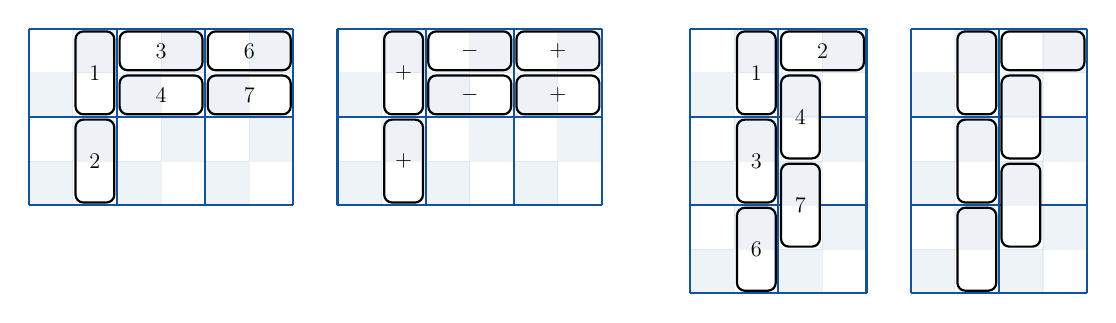
\begin{tikzpicture}[tableau, scale=.56]\gridLines{2}{3}\verticalDomino{1}{2}{1}\verticalDomino{3}{2}{2}\horizontalDomino{1}{3}{3}\horizontalDomino{2}{3}{4}\horizontalDomino{1}{5}{6}\horizontalDomino{2}{5}{7}\fixedSquaresForGrid{2}{3}\gridLinesShift{2}{3}{7}\verticalDominoShift{1}{2}{+}{7}\verticalDominoShift{3}{2}{+}{7}\horizontalDominoShift{1}{3}{-}{7}\horizontalDominoShift{2}{3}{-}{7}\horizontalDominoShift{1}{5}{+}{7}\horizontalDominoShift{2}{5}{+}{7}\fixedSquaresForGridShift{2}{3}{7}\gridLinesShift{3}{2}{15}\verticalDominoShift{1}{2}{1}{15}\horizontalDominoShift{1}{3}{2}{15}\verticalDominoShift{3}{2}{3}{15}\verticalDominoShift{2}{3}{4}{15}\verticalDominoShift{5}{2}{6}{15}\verticalDominoShift{4}{3}{7}{15}\fixedSquaresForGridShift{3}{2}{15}\gridLinesShift{3}{2}{20}\verticalDominoShift{1}{2}{}{20}\horizontalDominoShift{1}{3}{}{20}\verticalDominoShift{3}{2}{}{20}\verticalDominoShift{2}{3}{}{20}\verticalDominoShift{5}{2}{}{20}\verticalDominoShift{4}{3}{}{20}\fixedSquaresForGridShiftAlt{3}{2}{20}\end{tikzpicture}
      \end{figure}
      goes to
      \begin{figure}[H]
        % 1+ 2+ 3- 4- 6+ 7+ 5_8
        \centering
        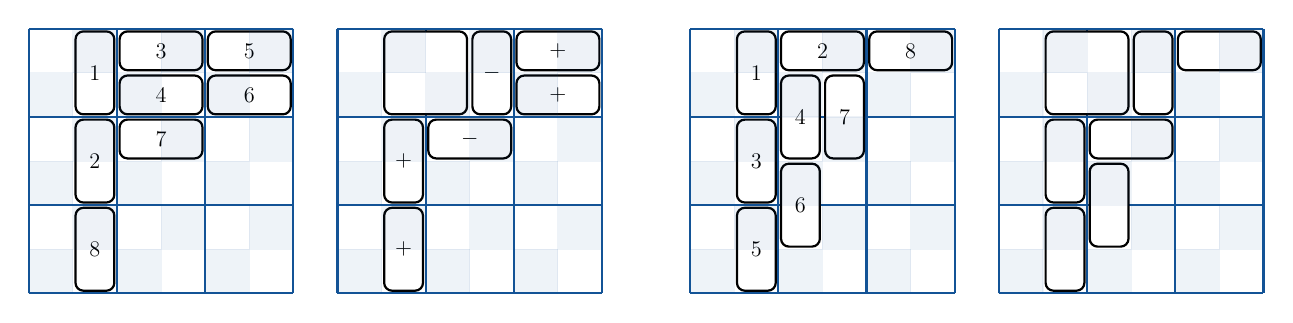
\begin{tikzpicture}[tableau, scale=.56]\gridLines{3}{3}\verticalDomino{1}{2}{1}\verticalDomino{3}{2}{2}\horizontalDomino{1}{3}{3}\horizontalDomino{2}{3}{4}\horizontalDomino{1}{5}{5}\horizontalDomino{2}{5}{6}\horizontalDomino{3}{3}{7}\verticalDomino{5}{2}{8}\fixedSquaresForGrid{3}{3}\gridLinesShift{3}{3}{7}\verticalDominoShift{3}{2}{+}{7}\verticalDominoShift{1}{4}{-}{7}\horizontalDominoShift{1}{5}{+}{7}\horizontalDominoShift{2}{5}{+}{7}\horizontalDominoShift{3}{3}{-}{7}\emptyBoxShift{1}{2}{7}\verticalDominoShift{5}{2}{+}{7}\fixedSquaresForGridShift{3}{3}{7}\gridLinesShift{3}{3}{15}\verticalDominoShift{1}{2}{1}{15}\horizontalDominoShift{1}{3}{2}{15}\verticalDominoShift{3}{2}{3}{15}\verticalDominoShift{2}{3}{4}{15}\verticalDominoShift{5}{2}{5}{15}\verticalDominoShift{4}{3}{6}{15}\verticalDominoShift{2}{4}{7}{15}\horizontalDominoShift{1}{5}{8}{15}\fixedSquaresForGridShift{3}{3}{15}\gridLinesShift{3}{3}{22}\verticalDominoShift{1}{4}{}{22}\verticalDominoShift{3}{2}{}{22}\verticalDominoShift{5}{2}{}{22}\verticalDominoShift{4}{3}{}{22}\horizontalDominoShift{3}{3}{}{22}\emptyBoxShift{1}{2}{22}\horizontalDominoShift{1}{5}{}{22}\fixedSquaresForGridShiftAlt{3}{3}{22}\end{tikzpicture}
      \end{figure}

      \item Here we are closing a boxed Type II cycle (which therefore contains just one domino, the one directly above this one).
      So, we are interested in four dominoes to start with, namely the cycle top and bottom and the two paired dominoes.
      There are five possible configurations for how these four dominoes are filled with signs.

      I think, again, we don't care that much what sign we put in if the side domino is blank, since that sign will be blanked when the next domino is added to the next row.
      However, we might need the tableau to be in a consistent state for the next domino to be added.
      Luckily, I have notes about that now.

      Another issue is that, if the top domino is blank, and if the sign we are adding does not end up being blanked, then we are adding a sign to that column which may be incompatible with whatever is above the top domino.
      So we need to bring that sign down first.

      Also, after adding a sign, we may be able to move it up in its column.

      Let's look at the cases.
      In all the cases, after we add the dominoes, we box them up.
      \begin{itemize}
        \item If the side domino is blank, we can add a horizontal domino here with either sign.
        The sign will be blanked when the next domino is added.
        For convenience, if the top domino has a sign, or if any domino in its column has as sign, we choose that sign.
        Otherwise we choose a random sign.
        As above, if the side domino is blank, we call
        \texttt{makeSpaceFor()} before adding the domino.
        (TODO pictures.)

        \item Here the side domino is vertical and has a sign and there is a blank domino in its column.
        We need to move the blank domino up.
        We do this using \texttt{findRowToAddSignX()}, with the variation that we will not be moving through cycles in the number tableaux at this location.
        (The cycles are already closed.)
        However, if \texttt{findRowToAddSignX()} makes a shape change in the sign tableaux, we will add the signed domino in the dual sign tableau.

        Basically, if there is a shape change, then we switch sides and do this situation, but on the other side.
        However, if we do that, then in one specific case, we could have another shape change and end up back on this side.
        Instead of doing that, we handle that as a special case,
        before calling \texttt{findRowToAddSignX()}.
        This will be the first case listed.

        Let's do the cases.
        \begin{itemize}
          \item Here the side domino has a $+$ (for convenience) sign, the top domino is blank, the top domino's row has a minus sign in it.
          On the dual side, the top corner domino has an $s$ (for convenience), and there is an $s$ sign in its row.
          Before calling  \texttt{findRowToAddSignX()}, we pull the $-$ sign intto the top domino.
          (Note, if we didn't do this, we could instead proceed to the next case.
          But, then we would end up having two shape changes.)
          \begin{figure}[H]
            \centering
            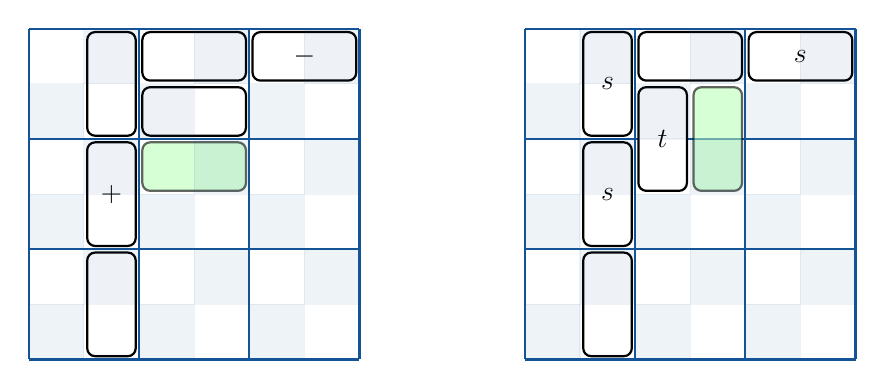
\begin{tikzpicture}[tableau, scale=.7]
              \gridLinesShift{3}{3}{7}\verticalDominoShift{1}{2}{}{7}\verticalDominoShift{3}{2}{+}{7}\verticalDominoShift{5}{2}{}{7}\horizontalDominoShift{1}{3}{}{7}\horizontalDominoShift{2}{3}{}{7}
              \horizontalDominoShift{1}{5}{-}{7}
              \horizontalDominoRSShift{3}{3}{}{7}
              \fixedSquaresForGridShift{3}{3}{7}
              \gridLinesShift{3}{3}{16}\verticalDominoShift{1}{2}{s}{16}\horizontalDominoShift{1}{3}{}{16}\horizontalDominoShift{1}{5}{s}{16}\verticalDominoShift{3}{2}{s}{16}\verticalDominoShift{2}{3}{t}{16}
              \verticalDominoShift{5}{2}{}{16}
              \verticalDominoRSShift{2}{4}{}{16}
              \fixedSquaresForGridShiftAlt{3}{3}{16}
            \end{tikzpicture}
          \end{figure}
          goes to
          \begin{figure}[H]
            \centering
            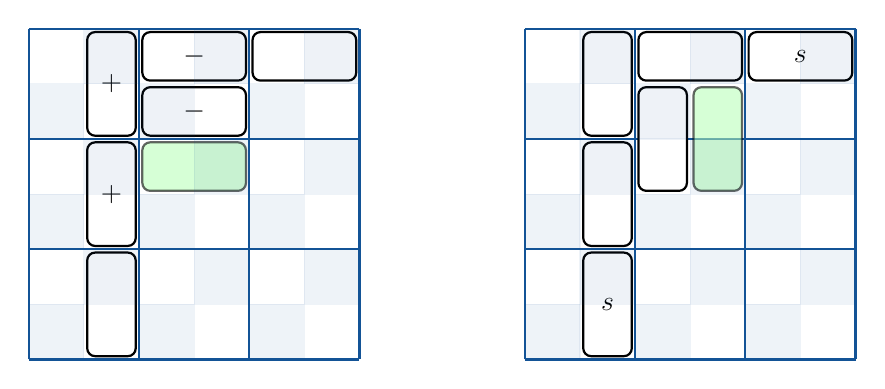
\begin{tikzpicture}[tableau, scale=.7]
              \gridLinesShift{3}{3}{7}
              \verticalDominoShift{1}{2}{+}{7}
              \verticalDominoShift{3}{2}{+}{7}
              \verticalDominoShift{5}{2}{}{7}
              \horizontalDominoShift{1}{3}{-}{7}
              \horizontalDominoShift{2}{3}{-}{7}
              \horizontalDominoShift{1}{5}{}{7}
              \horizontalDominoRSShift{3}{3}{}{7}
              \fixedSquaresForGridShift{3}{3}{7}

              \gridLinesShift{3}{3}{16}
              \verticalDominoShift{1}{2}{}{16}
              \horizontalDominoShift{1}{3}{}{16}
              \horizontalDominoShift{1}{5}{s}{16}
              \verticalDominoShift{3}{2}{}{16}
              \verticalDominoShift{2}{3}{}{16}
              \verticalDominoShift{5}{2}{s}{16}
              \verticalDominoRSShift{2}{4}{}{16}
              \fixedSquaresForGridShiftAlt{3}{3}{16}
            \end{tikzpicture}
          \end{figure}
          goes to
          \begin{figure}[H]
            \centering
            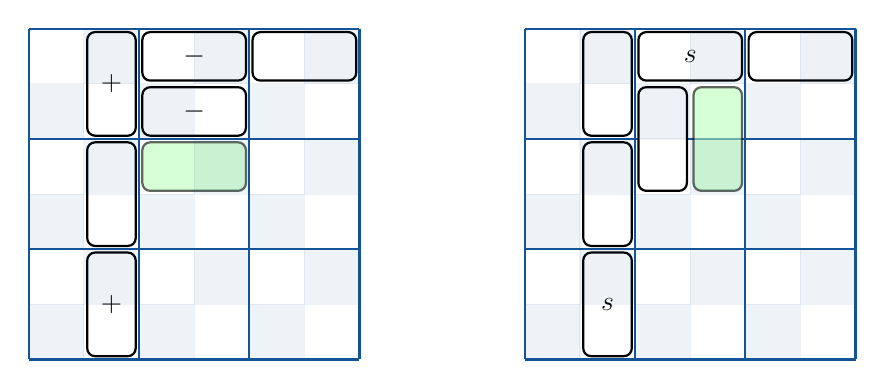
\begin{tikzpicture}[tableau, scale=.7]
              \gridLinesShift{3}{3}{7}
              \verticalDominoShift{1}{2}{+}{7}
              \verticalDominoShift{3}{2}{}{7}
              \verticalDominoShift{5}{2}{+}{7}
              \horizontalDominoShift{1}{3}{-}{7}
              \horizontalDominoShift{2}{3}{-}{7}
              \horizontalDominoShift{1}{5}{}{7}
              \horizontalDominoRSShift{3}{3}{}{7}
              \fixedSquaresForGridShift{3}{3}{7}

              \gridLinesShift{3}{3}{16}
              \verticalDominoShift{1}{2}{}{16}
              \horizontalDominoShift{1}{3}{s}{16}
              \horizontalDominoShift{1}{5}{}{16}
              \verticalDominoShift{3}{2}{}{16}
              \verticalDominoShift{2}{3}{}{16}
              \verticalDominoShift{5}{2}{s}{16}
              \verticalDominoRSShift{2}{4}{}{16}
              \fixedSquaresForGridShiftAlt{3}{3}{16}
            \end{tikzpicture}
          \end{figure}
          \begin{figure}[H]
            % 1+ 2+ 3s 5- 6s 7-
            \centering
            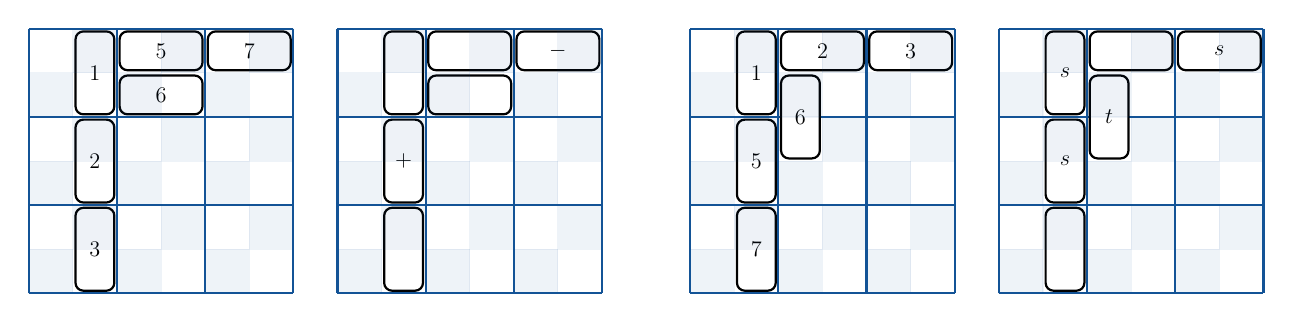
\begin{tikzpicture}[tableau, scale=.56]\gridLines{3}{3}\verticalDomino{1}{2}{1}\verticalDomino{3}{2}{2}\verticalDomino{5}{2}{3}\horizontalDomino{1}{3}{5}\horizontalDomino{2}{3}{6}\horizontalDomino{1}{5}{7}\fixedSquaresForGrid{3}{3}\gridLinesShift{3}{3}{7}\verticalDominoShift{1}{2}{}{7}\verticalDominoShift{3}{2}{+}{7}\verticalDominoShift{5}{2}{}{7}\horizontalDominoShift{1}{3}{}{7}\horizontalDominoShift{2}{3}{}{7}\horizontalDominoShift{1}{5}{-}{7}\fixedSquaresForGridShift{3}{3}{7}\gridLinesShift{3}{3}{15}\verticalDominoShift{1}{2}{1}{15}\horizontalDominoShift{1}{3}{2}{15}\horizontalDominoShift{1}{5}{3}{15}\verticalDominoShift{3}{2}{5}{15}\verticalDominoShift{2}{3}{6}{15}\verticalDominoShift{5}{2}{7}{15}\fixedSquaresForGridShift{3}{3}{15}\gridLinesShift{3}{3}{22}\verticalDominoShift{1}{2}{s}{22}\horizontalDominoShift{1}{3}{}{22}\horizontalDominoShift{1}{5}{s}{22}\verticalDominoShift{3}{2}{s}{22}\verticalDominoShift{2}{3}{t}{22}\verticalDominoShift{5}{2}{}{22}\fixedSquaresForGridShiftAlt{3}{3}{22}\end{tikzpicture}
          \end{figure}
          goes to
          \begin{figure}[H]
            % 1+ 2+ 3s 5- 6s 7- 4_8
            \centering
            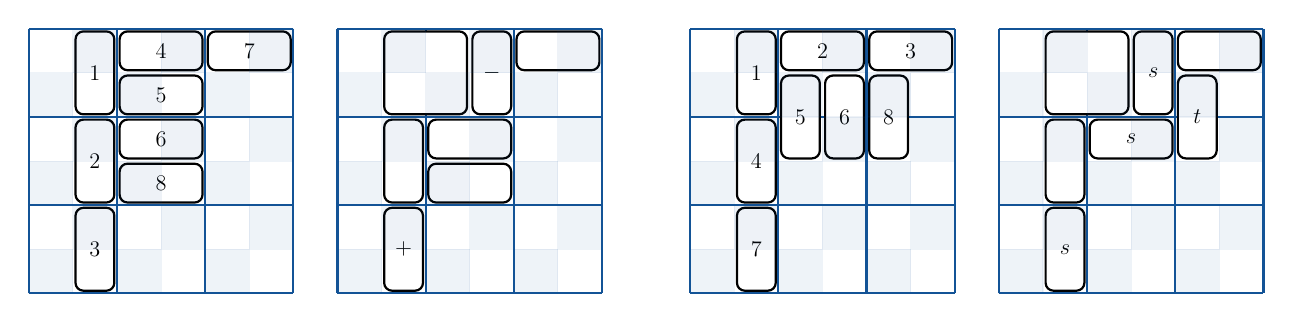
\begin{tikzpicture}[tableau, scale=.56]\gridLines{3}{3}\verticalDomino{1}{2}{1}\verticalDomino{3}{2}{2}\verticalDomino{5}{2}{3}\horizontalDomino{1}{3}{4}\horizontalDomino{2}{3}{5}\horizontalDomino{3}{3}{6}\horizontalDomino{1}{5}{7}\horizontalDomino{4}{3}{8}\fixedSquaresForGrid{3}{3}\gridLinesShift{3}{3}{7}\verticalDominoShift{3}{2}{}{7}\verticalDominoShift{5}{2}{+}{7}\verticalDominoShift{1}{4}{-}{7}\horizontalDominoShift{1}{5}{}{7}\horizontalDominoShift{3}{3}{}{7}\emptyBoxShift{1}{2}{7}\horizontalDominoShift{4}{3}{}{7}\fixedSquaresForGridShift{3}{3}{7}\gridLinesShift{3}{3}{15}\verticalDominoShift{1}{2}{1}{15}\horizontalDominoShift{1}{3}{2}{15}\horizontalDominoShift{1}{5}{3}{15}\verticalDominoShift{3}{2}{4}{15}\verticalDominoShift{2}{3}{5}{15}\verticalDominoShift{2}{4}{6}{15}\verticalDominoShift{5}{2}{7}{15}\verticalDominoShift{2}{5}{8}{15}\fixedSquaresForGridShift{3}{3}{15}\gridLinesShift{3}{3}{22}\verticalDominoShift{1}{4}{s}{22}\horizontalDominoShift{1}{5}{}{22}\verticalDominoShift{3}{2}{}{22}\verticalDominoShift{5}{2}{s}{22}\horizontalDominoShift{3}{3}{s}{22}\emptyBoxShift{1}{2}{22}\verticalDominoShift{2}{5}{t}{22}\fixedSquaresForGridShiftAlt{3}{3}{22}\end{tikzpicture}
          \end{figure}

          \item Here \texttt{findRowToAddSignX()} makes a shape change in the sign tableaux.
          So, basically, we are in the same situation as before, except on the other side.
          However, we know that the top domino has a sign.
          Our next step is to see if the side domino has a sign, and, if so, if we can bring up a blank domino.
          Note, this will not cause a shape change.
          We have eliminated that case in the previous case.
          Also note, this example ends up in the hard case.
          \begin{figure}[H]
            \centering
            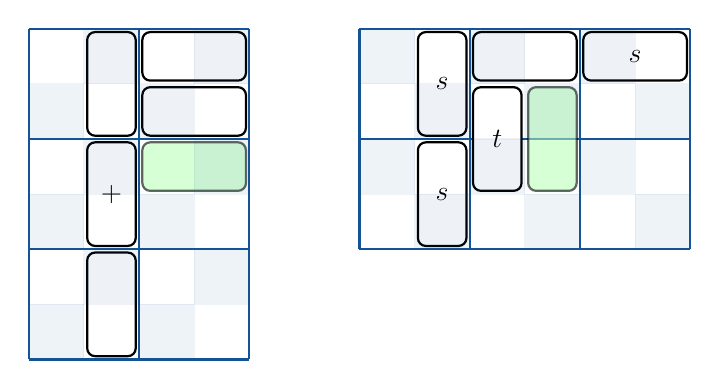
\begin{tikzpicture}[tableau, scale=.7]
              \gridLinesShift{3}{2}{5}
              \verticalDominoShift{1}{2}{}{5}
              \verticalDominoShift{3}{2}{+}{5}
              \verticalDominoShift{5}{2}{}{5}
              \horizontalDominoShift{1}{3}{}{5}
              \horizontalDominoShift{2}{3}{}{5}
              \horizontalDominoRSShift{3}{3}{}{5}
              \fixedSquaresForGridShift{3}{2}{5}

              \gridLinesShift{2}{3}{11}
              \verticalDominoShift{1}{2}{s}{11}
              \horizontalDominoShift{1}{3}{}{11}
              \horizontalDominoShift{1}{5}{s}{11}\verticalDominoShift{3}{2}{s}{11}
              \verticalDominoShift{2}{3}{t}{11}
              \verticalDominoRSShift{2}{4}{}{11}
              \fixedSquaresForGridShiftAlt{2}{3}{11}
            \end{tikzpicture}
          \end{figure}
          goes to
          \begin{figure}[H]
            \centering
            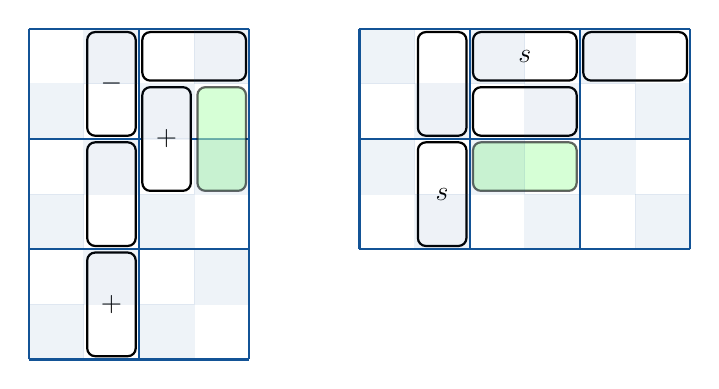
\begin{tikzpicture}[tableau, scale=.7]
              \gridLinesShift{3}{2}{5}
              \verticalDominoShift{1}{2}{-}{5}
              \verticalDominoShift{3}{2}{}{5}
              \verticalDominoShift{5}{2}{+}{5}
              \horizontalDominoShift{1}{3}{}{5}
              \verticalDominoShift{2}{3}{+}{5}
              \verticalDominoRSShift{2}{4}{}{5}
              \fixedSquaresForGridShift{3}{2}{5}

              \gridLinesShift{2}{3}{11}
              \verticalDominoShift{1}{2}{}{11}
              \horizontalDominoShift{1}{3}{s}{11}
              \horizontalDominoShift{1}{5}{}{11}
              \verticalDominoShift{3}{2}{s}{11}
              \horizontalDominoShift{2}{3}{}{11}
              \horizontalDominoRSShift{3}{3}{}{11}
              \fixedSquaresForGridShiftAlt{2}{3}{11}
            \end{tikzpicture}
          \end{figure}
          \begin{figure}[H]
            % 1+ 2+ 3s 5- 6s
            \centering
            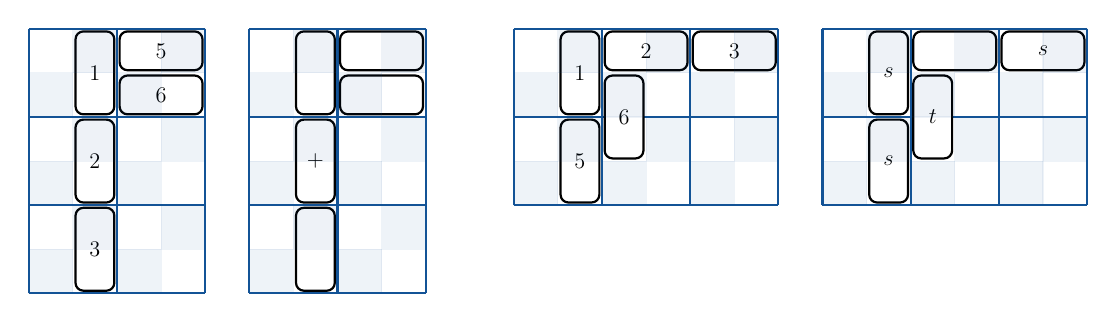
\begin{tikzpicture}[tableau, scale=.56]\gridLines{3}{2}\verticalDomino{1}{2}{1}\verticalDomino{3}{2}{2}\verticalDomino{5}{2}{3}\horizontalDomino{1}{3}{5}\horizontalDomino{2}{3}{6}\fixedSquaresForGrid{3}{2}\gridLinesShift{3}{2}{5}\verticalDominoShift{1}{2}{}{5}\verticalDominoShift{3}{2}{+}{5}\verticalDominoShift{5}{2}{}{5}\horizontalDominoShift{1}{3}{}{5}\horizontalDominoShift{2}{3}{}{5}\fixedSquaresForGridShift{3}{2}{5}\gridLinesShift{2}{3}{11}\verticalDominoShift{1}{2}{1}{11}\horizontalDominoShift{1}{3}{2}{11}\horizontalDominoShift{1}{5}{3}{11}\verticalDominoShift{3}{2}{5}{11}\verticalDominoShift{2}{3}{6}{11}\fixedSquaresForGridShift{2}{3}{11}\gridLinesShift{2}{3}{18}\verticalDominoShift{1}{2}{s}{18}\horizontalDominoShift{1}{3}{}{18}\horizontalDominoShift{1}{5}{s}{18}\verticalDominoShift{3}{2}{s}{18}\verticalDominoShift{2}{3}{t}{18}\fixedSquaresForGridShiftAlt{2}{3}{18}\end{tikzpicture}
          \end{figure}
          goes to
          \begin{figure}[H]
            % 1+ 2+ 3s 5- 6s 4_7
            \centering
            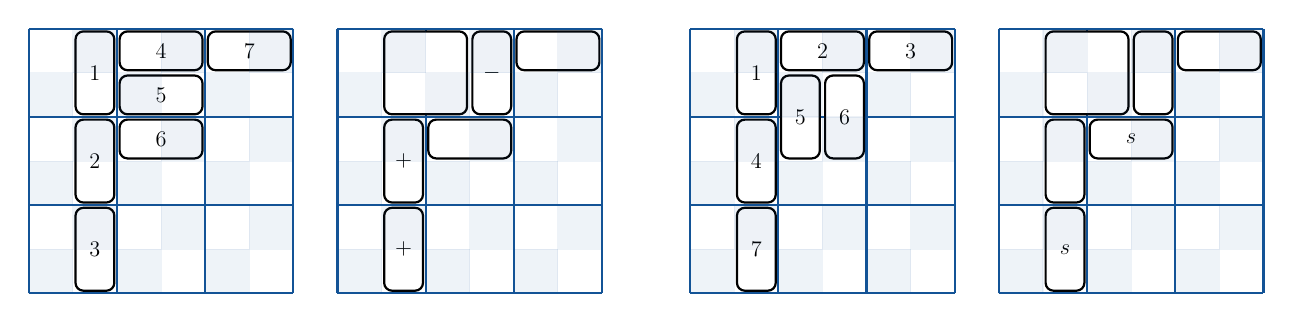
\begin{tikzpicture}[tableau, scale=.56]\gridLines{3}{3}\verticalDomino{1}{2}{1}\verticalDomino{3}{2}{2}\verticalDomino{5}{2}{3}\horizontalDomino{1}{3}{4}\horizontalDomino{2}{3}{5}\horizontalDomino{3}{3}{6}\horizontalDomino{1}{5}{7}\fixedSquaresForGrid{3}{3}\gridLinesShift{3}{3}{7}\verticalDominoShift{3}{2}{+}{7}\verticalDominoShift{5}{2}{+}{7}\verticalDominoShift{1}{4}{-}{7}\horizontalDominoShift{3}{3}{}{7}\emptyBoxShift{1}{2}{7}\horizontalDominoShift{1}{5}{}{7}\fixedSquaresForGridShift{3}{3}{7}\gridLinesShift{3}{3}{15}\verticalDominoShift{1}{2}{1}{15}\horizontalDominoShift{1}{3}{2}{15}\horizontalDominoShift{1}{5}{3}{15}\verticalDominoShift{3}{2}{4}{15}\verticalDominoShift{2}{3}{5}{15}\verticalDominoShift{2}{4}{6}{15}\verticalDominoShift{5}{2}{7}{15}\fixedSquaresForGridShift{3}{3}{15}\gridLinesShift{3}{3}{22}\verticalDominoShift{1}{4}{}{22}\horizontalDominoShift{1}{5}{}{22}\verticalDominoShift{3}{2}{}{22}\horizontalDominoShift{3}{3}{s}{22}\emptyBoxShift{1}{2}{22}\verticalDominoShift{5}{2}{s}{22}\fixedSquaresForGridShiftAlt{3}{3}{22}\end{tikzpicture}
          \end{figure}

          \item Otherwise, we can just proceed as if there was a blank in the side domino from the beginning.
        \end{itemize}

        \item Here the side domino is vertical and has a sign ($+$ for convenience) and there are no blank signs in its column.
        So, basically, we just put a $-$ sign in the newly-added domino.
        There are two cases where that causes problems.
        One is where the top domino also contains a $+$ sign.
        The other is when the top domino is blank, and the column above it has a $+$ sign.
        Let's see the base case and these special cases.
        \begin{itemize}
          \item Here is an easy case:
          \begin{figure}[H]
            % 1+ 2+ 4- 5-
            \centering
            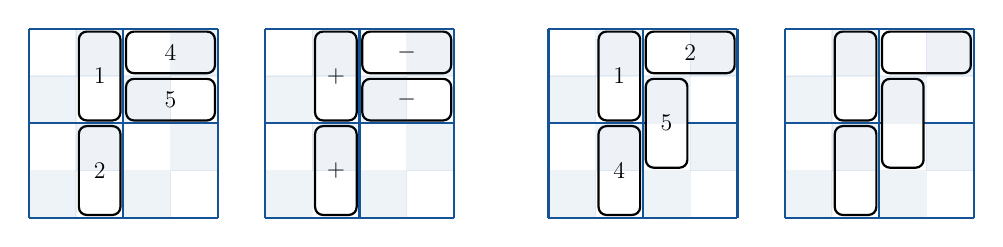
\begin{tikzpicture}[tableau, scale=.6]\gridLines{2}{2}\verticalDomino{1}{2}{1}\verticalDomino{3}{2}{2}\horizontalDomino{1}{3}{4}\horizontalDomino{2}{3}{5}\fixedSquaresForGrid{2}{2}\gridLinesShift{2}{2}{5}\verticalDominoShift{1}{2}{+}{5}\verticalDominoShift{3}{2}{+}{5}\horizontalDominoShift{1}{3}{-}{5}\horizontalDominoShift{2}{3}{-}{5}\fixedSquaresForGridShift{2}{2}{5}\gridLinesShift{2}{2}{11}\verticalDominoShift{1}{2}{1}{11}\horizontalDominoShift{1}{3}{2}{11}\verticalDominoShift{3}{2}{4}{11}\verticalDominoShift{2}{3}{5}{11}\fixedSquaresForGridShift{2}{2}{11}\gridLinesShift{2}{2}{16}\verticalDominoShift{1}{2}{}{16}\horizontalDominoShift{1}{3}{}{16}\verticalDominoShift{3}{2}{}{16}\verticalDominoShift{2}{3}{}{16}\fixedSquaresForGridShiftAlt{2}{2}{16}\end{tikzpicture}
          \end{figure}
          goes to
          \begin{figure}[H]
            % 1+ 2+ 4- 5- 3_6
            \centering
            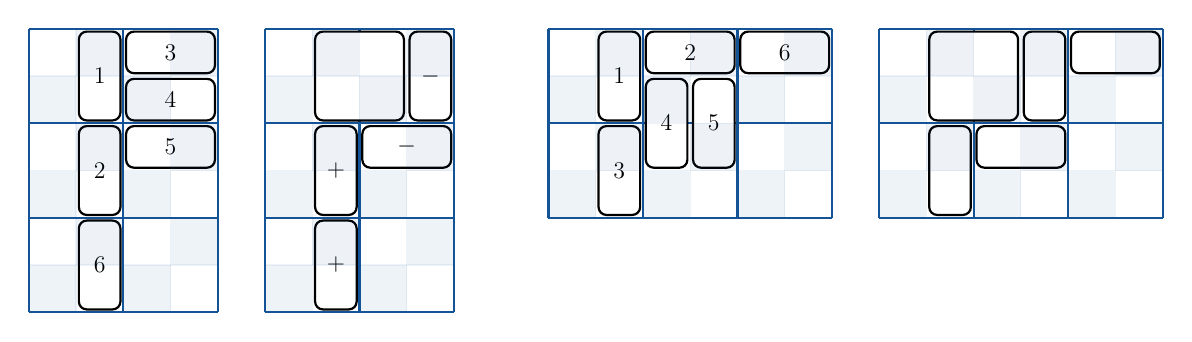
\begin{tikzpicture}[tableau, scale=.6]\gridLines{3}{2}\verticalDomino{1}{2}{1}\verticalDomino{3}{2}{2}\horizontalDomino{1}{3}{3}\horizontalDomino{2}{3}{4}\horizontalDomino{3}{3}{5}\verticalDomino{5}{2}{6}\fixedSquaresForGrid{3}{2}\gridLinesShift{3}{2}{5}\verticalDominoShift{3}{2}{+}{5}\verticalDominoShift{1}{4}{-}{5}\horizontalDominoShift{3}{3}{-}{5}\emptyBoxShift{1}{2}{5}\verticalDominoShift{5}{2}{+}{5}\fixedSquaresForGridShift{3}{2}{5}\gridLinesShift{2}{3}{11}\verticalDominoShift{1}{2}{1}{11}\horizontalDominoShift{1}{3}{2}{11}\verticalDominoShift{3}{2}{3}{11}\verticalDominoShift{2}{3}{4}{11}\verticalDominoShift{2}{4}{5}{11}\horizontalDominoShift{1}{5}{6}{11}\fixedSquaresForGridShift{2}{3}{11}\gridLinesShift{2}{3}{18}\verticalDominoShift{1}{4}{}{18}\verticalDominoShift{3}{2}{}{18}\horizontalDominoShift{3}{3}{}{18}\emptyBoxShift{1}{2}{18}\horizontalDominoShift{1}{5}{}{18}\fixedSquaresForGridShiftAlt{2}{3}{18}\end{tikzpicture}
          \end{figure}
          \item Here there is a blank domino in the column above.  The newly-added domino can move up.
          \begin{figure}[H]
            % 1+ 2s 3t 6_7 5_8
            \centering
            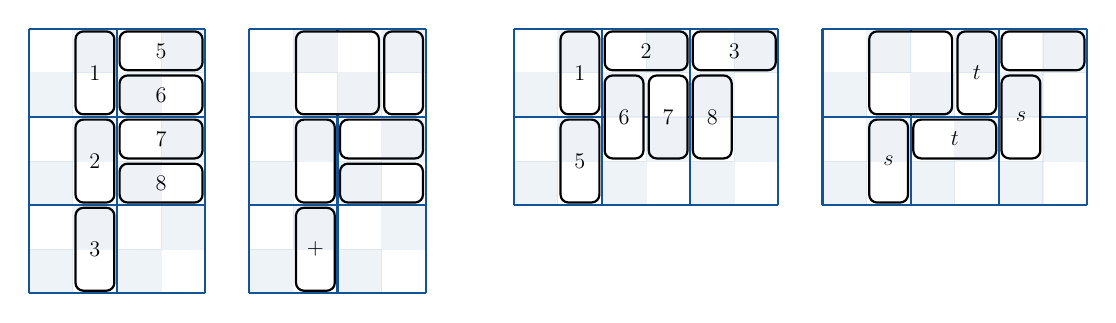
\begin{tikzpicture}[tableau, scale=.56]\gridLines{3}{2}\verticalDomino{1}{2}{1}\verticalDomino{3}{2}{2}\verticalDomino{5}{2}{3}\horizontalDomino{1}{3}{5}\horizontalDomino{2}{3}{6}\horizontalDomino{3}{3}{7}\horizontalDomino{4}{3}{8}\fixedSquaresForGrid{3}{2}\gridLinesShift{3}{2}{5}\verticalDominoShift{3}{2}{}{5}\verticalDominoShift{5}{2}{+}{5}\verticalDominoShift{1}{4}{}{5}\horizontalDominoShift{3}{3}{}{5}\emptyBoxShift{1}{2}{5}\horizontalDominoShift{4}{3}{}{5}\fixedSquaresForGridShift{3}{2}{5}\gridLinesShift{2}{3}{11}\verticalDominoShift{1}{2}{1}{11}\horizontalDominoShift{1}{3}{2}{11}\horizontalDominoShift{1}{5}{3}{11}\verticalDominoShift{3}{2}{5}{11}\verticalDominoShift{2}{3}{6}{11}\verticalDominoShift{2}{4}{7}{11}\verticalDominoShift{2}{5}{8}{11}\fixedSquaresForGridShift{2}{3}{11}\gridLinesShift{2}{3}{18}\verticalDominoShift{1}{4}{t}{18}\horizontalDominoShift{1}{5}{}{18}\verticalDominoShift{3}{2}{s}{18}\horizontalDominoShift{3}{3}{t}{18}\emptyBoxShift{1}{2}{18}\verticalDominoShift{2}{5}{s}{18}\fixedSquaresForGridShiftAlt{2}{3}{18}\end{tikzpicture}
          \end{figure}
          goes to
          \begin{figure}[H]
            % 1+ 2s 3t 6_7 5_8 4_9
            \centering
            \begin{tikzpicture}[tableau, scale=.56]\gridLines{4}{2}\verticalDomino{1}{2}{1}\verticalDomino{3}{2}{2}\verticalDomino{5}{2}{3}\horizontalDomino{1}{3}{4}\horizontalDomino{2}{3}{5}\horizontalDomino{3}{3}{6}\horizontalDomino{4}{3}{7}\horizontalDomino{5}{3}{8}\verticalDomino{7}{2}{9}\fixedSquaresForGrid{4}{2}\gridLinesShift{4}{2}{5}\verticalDominoShift{5}{2}{+}{5}\verticalDominoShift{1}{4}{-}{5}\verticalDominoShift{3}{4}{}{5}\emptyBoxShift{1}{2}{5}\horizontalDominoShift{5}{3}{}{5}\emptyBoxShift{3}{2}{5}\verticalDominoShift{7}{2}{+}{5}\fixedSquaresForGridShift{4}{2}{5}\gridLinesShift{2}{4}{11}\verticalDominoShift{1}{2}{1}{11}\horizontalDominoShift{1}{3}{2}{11}\horizontalDominoShift{1}{5}{3}{11}\verticalDominoShift{3}{2}{4}{11}\verticalDominoShift{2}{3}{5}{11}\verticalDominoShift{2}{4}{6}{11}\verticalDominoShift{2}{5}{7}{11}\verticalDominoShift{2}{6}{8}{11}\horizontalDominoShift{1}{7}{9}{11}\fixedSquaresForGridShift{2}{4}{11}\gridLinesShift{2}{4}{20}\verticalDominoShift{1}{6}{}{20}\verticalDominoShift{3}{2}{}{20}\horizontalDominoShift{3}{3}{s}{20}\emptyBoxShift{1}{2}{20}\horizontalDominoShift{3}{5}{t}{20}\emptyBoxShift{1}{4}{20}\horizontalDominoShift{1}{7}{}{20}\fixedSquaresForGridShiftAlt{2}{4}{20}\end{tikzpicture}
          \end{figure}
          \item Here the top domino also contains a $+$ sign.
          Here we basically undo what was done when two signs on the dual side were trapped by the two $+$ signs.
          We free them and separate them.
          On the left, the $-$ sign combines with one of the $+$ signs, and they disappear, leaving only one $+$ sign, in the middle.
          First, a basic example.
          \begin{figure}[H]
            % 1s 2t 4+ 5+
            \centering
            \begin{tikzpicture}[tableau, scale=.56]\gridLines{2}{2}\verticalDomino{1}{2}{1}\verticalDomino{3}{2}{2}\horizontalDomino{1}{3}{4}\horizontalDomino{2}{3}{5}\fixedSquaresForGrid{2}{2}\gridLinesShift{2}{2}{5}\verticalDominoShift{1}{2}{}{5}\verticalDominoShift{3}{2}{+}{5}\horizontalDominoShift{1}{3}{+}{5}\horizontalDominoShift{2}{3}{}{5}\fixedSquaresForGridShift{2}{2}{5}\gridLinesShift{2}{2}{11}\verticalDominoShift{1}{2}{1}{11}\horizontalDominoShift{1}{3}{2}{11}\verticalDominoShift{3}{2}{4}{11}\verticalDominoShift{2}{3}{5}{11}\fixedSquaresForGridShift{2}{2}{11}\gridLinesShift{2}{2}{16}\verticalDominoShift{1}{2}{t}{16}\horizontalDominoShift{1}{3}{}{16}\verticalDominoShift{3}{2}{}{16}\verticalDominoShift{2}{3}{s}{16}\fixedSquaresForGridShiftAlt{2}{2}{16}\end{tikzpicture}
          \end{figure}
          \begin{figure}[H]
            % 1s 2t 4+ 5+ 3_6
            \centering
            \begin{tikzpicture}[tableau, scale=.56]\gridLines{3}{2}\verticalDomino{1}{2}{1}\verticalDomino{3}{2}{2}\horizontalDomino{1}{3}{3}\horizontalDomino{2}{3}{4}\horizontalDomino{3}{3}{5}\verticalDomino{5}{2}{6}\fixedSquaresForGrid{3}{2}\gridLinesShift{3}{2}{5}\verticalDominoShift{3}{2}{}{5}\verticalDominoShift{1}{4}{}{5}\horizontalDominoShift{3}{3}{+}{5}\emptyBoxShift{1}{2}{5}\verticalDominoShift{5}{2}{+}{5}\fixedSquaresForGridShift{3}{2}{5}\gridLinesShift{2}{3}{11}\verticalDominoShift{1}{2}{1}{11}\horizontalDominoShift{1}{3}{2}{11}\verticalDominoShift{3}{2}{3}{11}\verticalDominoShift{2}{3}{4}{11}\verticalDominoShift{2}{4}{5}{11}\horizontalDominoShift{1}{5}{6}{11}\fixedSquaresForGridShift{2}{3}{11}\gridLinesShift{2}{3}{18}\verticalDominoShift{1}{4}{t}{18}\verticalDominoShift{3}{2}{s}{18}\horizontalDominoShift{3}{3}{}{18}\emptyBoxShift{1}{2}{18}\horizontalDominoShift{1}{5}{}{18}\fixedSquaresForGridShiftAlt{2}{3}{18}\end{tikzpicture}
          \end{figure}
          Note, the $t$ is in a row of all blanks, by our assumption that the side column on the $+$ side had all $+$ signs.
          The easy issue is that we need to make space for the lower sign
          \item Here the top domino is blank, and the column above it has a $+$ sign.
          We move it down first.
          Then we are in the previous case.
          \begin{figure}[H]
            % 1s 2t 3s 6+ 7+ 5_8
            \centering
            \begin{tikzpicture}[tableau, scale=.56]\gridLines{3}{2}\verticalDomino{1}{2}{1}\verticalDomino{3}{2}{2}\verticalDomino{5}{2}{3}\horizontalDomino{1}{3}{5}\horizontalDomino{2}{3}{6}\horizontalDomino{3}{3}{7}\horizontalDomino{4}{3}{8}\fixedSquaresForGrid{3}{2}\gridLinesShift{3}{2}{5}\verticalDominoShift{3}{2}{}{5}\verticalDominoShift{5}{2}{+}{5}\verticalDominoShift{1}{4}{+}{5}\horizontalDominoShift{3}{3}{}{5}\emptyBoxShift{1}{2}{5}\horizontalDominoShift{4}{3}{}{5}\fixedSquaresForGridShift{3}{2}{5}\gridLinesShift{2}{3}{11}\verticalDominoShift{1}{2}{1}{11}\horizontalDominoShift{1}{3}{2}{11}\horizontalDominoShift{1}{5}{3}{11}\verticalDominoShift{3}{2}{5}{11}\verticalDominoShift{2}{3}{6}{11}\verticalDominoShift{2}{4}{7}{11}\verticalDominoShift{2}{5}{8}{11}\fixedSquaresForGridShift{2}{3}{11}\gridLinesShift{2}{3}{18}\verticalDominoShift{1}{4}{s}{18}\horizontalDominoShift{1}{5}{}{18}\verticalDominoShift{3}{2}{}{18}\horizontalDominoShift{3}{3}{s}{18}\emptyBoxShift{1}{2}{18}\verticalDominoShift{2}{5}{t}{18}\fixedSquaresForGridShiftAlt{2}{3}{18}\end{tikzpicture}
          \end{figure}
          goes to
          \begin{figure}[H]
            % 1s 2t 3s 6+ 7+ 5_8
            \centering
            \begin{tikzpicture}[tableau, scale=.56]\gridLines{3}{2}\verticalDomino{1}{2}{1}\verticalDomino{3}{2}{2}\verticalDomino{5}{2}{3}\horizontalDomino{1}{3}{5}\horizontalDomino{2}{3}{6}\horizontalDomino{3}{3}{7}\horizontalDomino{4}{3}{8}\fixedSquaresForGrid{3}{2}
            \gridLinesShift{3}{2}{5}\verticalDominoShift{3}{2}{}{5}\verticalDominoShift{5}{2}{+}{5}\verticalDominoShift{1}{4}{}{5}\horizontalDominoShift{3}{3}{+}{5}\emptyBoxShift{1}{2}{5}\horizontalDominoShift{4}{3}{}{5}\fixedSquaresForGridShift{3}{2}{5}
            \gridLinesShift{2}{3}{11}\verticalDominoShift{1}{2}{1}{11}\horizontalDominoShift{1}{3}{2}{11}\horizontalDominoShift{1}{5}{3}{11}\verticalDominoShift{3}{2}{5}{11}\verticalDominoShift{2}{3}{6}{11}\verticalDominoShift{2}{4}{7}{11}\verticalDominoShift{2}{5}{8}{11}\fixedSquaresForGridShift{2}{3}{11}
            \gridLinesShift{2}{3}{18}\verticalDominoShift{1}{4}{s}{18}\horizontalDominoShift{1}{5}{}{18}\verticalDominoShift{3}{2}{s}{18}\horizontalDominoShift{3}{3}{}{18}\emptyBoxShift{1}{2}{18}\verticalDominoShift{2}{5}{t}{18}\fixedSquaresForGridShiftAlt{2}{3}{18}\end{tikzpicture}
          \end{figure}
          goes to
          \begin{figure}[H]
            % 1s 2t 3s 6+ 7+ 5_8 4_9
            \centering
            \begin{tikzpicture}[tableau, scale=.56]\gridLines{4}{2}\verticalDomino{1}{2}{1}\verticalDomino{3}{2}{2}\verticalDomino{5}{2}{3}\horizontalDomino{1}{3}{4}\horizontalDomino{2}{3}{5}\horizontalDomino{3}{3}{6}\horizontalDomino{4}{3}{7}\horizontalDomino{5}{3}{8}\verticalDomino{7}{2}{9}\fixedSquaresForGrid{4}{2}\gridLinesShift{4}{2}{5}\verticalDominoShift{5}{2}{}{5}\verticalDominoShift{1}{4}{}{5}\verticalDominoShift{3}{4}{}{5}\emptyBoxShift{1}{2}{5}\horizontalDominoShift{5}{3}{+}{5}\emptyBoxShift{3}{2}{5}\verticalDominoShift{7}{2}{+}{5}\fixedSquaresForGridShift{4}{2}{5}\gridLinesShift{2}{4}{11}\verticalDominoShift{1}{2}{1}{11}\horizontalDominoShift{1}{3}{2}{11}\horizontalDominoShift{1}{5}{3}{11}\verticalDominoShift{3}{2}{4}{11}\verticalDominoShift{2}{3}{5}{11}\verticalDominoShift{2}{4}{6}{11}\verticalDominoShift{2}{5}{7}{11}\verticalDominoShift{2}{6}{8}{11}\horizontalDominoShift{1}{7}{9}{11}\fixedSquaresForGridShift{2}{4}{11}\gridLinesShift{2}{4}{20}\verticalDominoShift{1}{6}{s}{20}\verticalDominoShift{3}{2}{s}{20}\horizontalDominoShift{3}{3}{t}{20}\emptyBoxShift{1}{2}{20}\horizontalDominoShift{3}{5}{}{20}\emptyBoxShift{1}{4}{20}\horizontalDominoShift{1}{7}{}{20}\fixedSquaresForGridShiftAlt{2}{4}{20}\end{tikzpicture}
          \end{figure}
        \end{itemize}

        \item Here the side domino is horizontal and has a $+$ sign.
        In this configuration, there is a column above the top domino on the dual side.
        Basically, we proceed as before, except in one case, which we'll describe.
        In this case, the top domino also contains a $+$ sign.
        Assume $s$ is in the top corner domino.
        If there is a $t$ in the column above the top domino, we can't proceed as usual.
        Instead, pull the $t$ down first.
        Now the side domino has no sign, and we can put the $-$ sign there, by swapping it with the blank corresponding to the $t$ domino.
        Now the $t$ domino is lower, so we need to call \texttt{makeSpaceFor()} for it.
        \begin{figure}[H]
          % 2+ 3- 4t 1_5 7+ 8+
          \centering
          \begin{tikzpicture}[tableau, scale=.56]\gridLines{2}{3}\horizontalDomino{1}{2}{1}\horizontalDomino{2}{2}{2}\verticalDomino{1}{4}{3}\verticalDomino{3}{2}{4}\horizontalDomino{3}{3}{5}\horizontalDomino{1}{5}{7}\horizontalDomino{2}{5}{8}\fixedSquaresForGrid{2}{3}\gridLinesShift{2}{3}{7}\verticalDominoShift{1}{4}{}{7}\verticalDominoShift{3}{2}{}{7}\emptyBoxShift{1}{2}{7}\horizontalDominoShift{3}{3}{+}{7}\horizontalDominoShift{1}{5}{+}{7}\horizontalDominoShift{2}{5}{}{7}\fixedSquaresForGridShift{2}{3}{7}\gridLinesShift{3}{2}{15}\verticalDominoShift{1}{2}{1}{15}\verticalDominoShift{1}{3}{2}{15}\verticalDominoShift{3}{2}{3}{15}\verticalDominoShift{1}{4}{4}{15}\horizontalDominoShift{3}{3}{5}{15}\verticalDominoShift{5}{2}{7}{15}\verticalDominoShift{4}{3}{8}{15}\fixedSquaresForGridShift{3}{2}{15}\gridLinesShift{3}{2}{20}\verticalDominoShift{3}{2}{s}{20}\verticalDominoShift{1}{4}{t}{20}\emptyBoxShift{1}{2}{20}\horizontalDominoShift{3}{3}{}{20}\verticalDominoShift{5}{2}{}{20}\verticalDominoShift{4}{3}{t}{20}\fixedSquaresForGridShiftAlt{3}{2}{20}\end{tikzpicture}
        \end{figure}
        \begin{figure}[H]
          % 2+ 3- 4t 1_5 7+ 8+ 6_9
          \centering
          \begin{tikzpicture}[tableau, scale=.56]\gridLines{3}{3}\horizontalDomino{1}{2}{1}\horizontalDomino{2}{2}{2}\verticalDomino{1}{4}{3}\verticalDomino{3}{2}{4}\horizontalDomino{3}{3}{5}\horizontalDomino{1}{5}{6}\horizontalDomino{2}{5}{7}\horizontalDomino{3}{5}{8}\verticalDomino{5}{2}{9}\fixedSquaresForGrid{3}{3}\gridLinesShift{3}{3}{7}\verticalDominoShift{3}{2}{+}{7}\emptyBoxShift{1}{2}{7}\horizontalDominoShift{3}{3}{-}{7}\verticalDominoShift{1}{6}{+}{7}\horizontalDominoShift{3}{5}{}{7}\emptyBoxShift{1}{4}{7}\verticalDominoShift{5}{2}{+}{7}\fixedSquaresForGridShift{3}{3}{7}\gridLinesShift{3}{3}{15}\verticalDominoShift{1}{2}{1}{15}\verticalDominoShift{1}{3}{2}{15}\verticalDominoShift{3}{2}{3}{15}\verticalDominoShift{1}{4}{4}{15}\horizontalDominoShift{3}{3}{5}{15}\verticalDominoShift{5}{2}{6}{15}\verticalDominoShift{4}{3}{7}{15}\verticalDominoShift{4}{4}{8}{15}\horizontalDominoShift{1}{5}{9}{15}\fixedSquaresForGridShift{3}{3}{15}\gridLinesShift{3}{3}{22}\verticalDominoShift{1}{4}{}{22}\emptyBoxShift{1}{2}{22}\verticalDominoShift{3}{4}{}{22}\verticalDominoShift{5}{2}{}{22}\horizontalDominoShift{5}{3}{t}{22}\emptyBoxShift{3}{2}{22}\horizontalDominoShift{1}{5}{}{22}\fixedSquaresForGridShiftAlt{3}{3}{22}\end{tikzpicture}
        \end{figure}
      \end{itemize}
    \end{itemize}
  \end{itemize}
\end{document}
